% !Mode:: "TeX:UTF-8"
%这样可以确保 .tex 文件默认使用 UTF-8 的格式打开

%学位论文怎么写,这位教授说的太好了!
%https://mp.weixin.qq.com/s/NbPkZWytwiu-nBysj4P9HQ

\def\usewhat{pdflatex}                              % 定义编译方式 dvipdfmx 或者 pdflatex ,默认为 dvipdfmx
                                                    % 方式编译,如果需要修改,只需改变花括号中的内容即可。
%\setlength{\baselineskip}{20pt}
%\setlength{\headheight}{25pt}
\documentclass[a4paper,12.5pt,openany,twoside]{book}
%openright, openany 指定新的一章\chapter 是在奇数页(右侧)开头,还是直接紧跟着上 一页开头。report 缺省为openany,book 缺省为openright。【对article 无效】


                                           % 如果论文超过60页 可以使用twoside 双面打印
\input{setup/package}                      % 定义本文所使用宏包
\graphicspath{{figures/}}                  % 定义所有的.eps文件在figures子目录下
\begin{document}                           % 开始全文
\begin{CJK*}{UTF8}{song}                   % 开始中文字体使用
\input{setup/format}                       % 完成对论文各个部分格式的设置
\frontmatter                               % 以下是论文导言部分,包括论文的封面,中英文摘要和中文目录
% !Mode:: "TeX:UTF-8"

\chnunumer{10532}
\chnuname{湖南大学}
\cclassnumber{TP391}
\cnumber{S151000891}
\csecret{普通}
\cmajor{计算机网络}
\cheading{硕士学位论文}      % 设置正文的页眉,以及自己的学位级别
\ctitle{SDN/NFV网络架构可生存性算法研究}  %封面用论文标题,自己可手动断行
\etitle{SDN/NFV Network Architecture Survivable Algorithm Research}
\caffil{信息科学与工程学院} %学院名称
\csubjecttitle{学科专业}
\csubject{计算机科学与技术}   %专业
\cauthortitle{研究生}     % 学位
\cauthor{陶恒}   %学生姓名
\ename{Tao~~Heng}
\cbe{M.E.~(Hunan University)~2018}
%\cms{M.S.~(Hunan University)2010}
\cdegree{thesis}
\cclass{Master of engineering}
\emajor{Computer Science and Technology}
\ehnu{Hunan~University}
\esupervisor{Kun Xie}
\csupervisortitle{指导教师}
\csupervisor{谢鲲~教授} %导师姓名
\elevel{Professor} %导师职称
\cchair{~~~~~~~~}
\ddate{~~~~~~~~年~~~~月~~~~日}
\edate{April,~2018}
\untitle{湖~~南~~大~~学}
\declaretitle{学位论文原创性声明}
\declarecontent{
本人郑重声明:所呈交的论文是本人在导师的指导下独立进行研究所取得的研究成果。除了文中特别加以标注引用的内容外,本论文不包含任何其他个人或集体已经发表或撰写的成果作品。对本文的研究做出重要贡献的个人和集体,均已在文中以明确方式标明。本人完全意识到本声明的法律后果由本人承担。
}
\authorizationtitle{学位论文版权使用授权书}
\authorizationcontent{
本学位论文作者完全了解学校有关保留、使用学位论文的规定,同意学校保留并向国家有关部门或机构送交论文的复印件和电子版,允许论文被查阅和借阅。本人授权湖南大学可以将本学位论文的全部或部分内容编入有关数据库进行检索,可以采用影印、缩印或扫描等复制手段保存和汇编本学位论文。
}
\authorizationadd{本学位论文属于}
\authorsigncap{作者签名:}
\supervisorsigncap{导师签名:}
\signdatecap{签字日期:}


%\cdate{\CJKdigits{\the\year} 年\CJKnumber{\the\month} 月 \CJKnumber{\the\day} 日}
% 如需改成二零一二年四月二十五日的格式,可以直接输入,即如下所示
% \cdate{二零一二年四月二十五日}
\cdate{~~~~~~~~年~~~~月~~~~日} % 此日期显示格式为阿拉伯数字 如2012 年4 月25 日
\cabstract{
现今网络规模越来越大,业务也在不断地扩展,传统的网络架构及技术己经无法满足快速配置、按需调动等要求,软件定义网络(SDN)就是为了应对现有网络无法解决的问题而被提出来的。为了使管理更加灵活高效,SDN架构将控制平面与转发平面进行了解耦分离,并且具有可编程特性。另外,利用网络功能虚拟化将网络资源进行虚拟化在很大程度上也可以解决现有网络无法解决的问题,用户的多个虚拟网络可以同时存在于一个底层物理网络上,它们依据不同的嵌入算法向底层物理网络映射,嵌入的虚拟网络会共享底层物理网络的资源。

SDN作为新型网络架构,控制层与转发层分离将推动实现传统网络无法实现或者较难实现的网络业务,传统网络的路由算法只在源节点和目的节点之间提供一条Qos路径,这一做法已不能满足在网络连接出现故障时保持业务持续不间断地进行这一可生存性保护需求。SDN在光网络和Overlay网络中高效实现分离路径算法,试图在源节点和目的节点之间寻找满足一定Qos 约束的分离路径(链路分离,节点分离或SRLG分离),一条主用路径,另一条备用路径。当主用路径出现故障时,将其承载的业务流转换到备用路径上,从而实现快速的业务恢复。因此,分离路径算法研究有很重要的实用价值。

SDN作为新型网络架构,网络虚拟化作为未来网络研究的重要领域,两者的结合具有很高的研究意义。现在看来,SDN 适合的领域应该是数据中心网络虚拟化的应用。在网络虚拟化过程中,不可避开的技术就是嵌入算法以及可生存性保护的研究,嵌入算法主要是考虑虚拟网络节点和链路向底层物理网络的映射,如何为虚 拟网络在底层物理网中找到满足条件且最优的路径;负责可生存性保护可以保证底层物理网资源失效的情况下,原本虚拟网络业务正常运行。

本文结合实际项目,基于SDN/NFV网络架构以可生存性算法作为课题的研究方向, 主要研究了以下四个方面的内容:

首先,研究网络可生存性技术,对网络故障失效环境进行了研究,并且探讨了已有各种情形的路径保护算法。

其次,光网络和Overlay网络中,考虑共享风险链路组分离的约束条件,在SRLG分离路由算法设计中,提出一个特殊的边分而治之集,通过创新的容量设置获得这个集合,分而治之的解决SRLG分离路由算法,并且都与己有算法进行了对比分析。

其次,研究SDN虚拟网络技术,对SDN网络虚拟化的环境进行了研究,并且探讨了虚拟网络向底层物理网进行映射时的不同嵌入算法和可生存性嵌入算法。

最后,在虚拟网络向底层物理网络映射时,考虑节点和链路的映射以及可生存性嵌入算法的设计,在可生存性嵌入算法的设计中,考虑到节点带有特定功能约束的条件,本文结合已有算法的不足,设计出虚拟网络分割嵌入的动态规划方法,并且都与己有算法进行了对比分析。

}
%中文摘要应将学位论文的内容要点简短明了地表达出来,约500~800字左右(限一页),字体为宋体小四号。内容应包括工作目的、研究方法、成果和结论。要突出本论文的创新点,语言力求精炼。为了便于文献检索,应在本页下方另起一行注明论文的关键词(3-7个)。
\ckeywords{软件定义网络;~~网络功能虚拟;~~分离路径;~~虚拟网络嵌入;~~可生存性}
\eabstract{The network size is growing, and the business is constantly expanding at present, thus resulting in that the traditional network architecture and technology have been unable to meet the on-demand transfer、rapid configuration and other requirements,then, SDN is put forward to deal with this situation. SDN is an innovative network architecture, in order to make the management more flexible, it's forwarding plane and control plane are independent of each other. What’s more,it has an excellent feature of good programming. In addition, virtualization of network resources can also solve this problem to a large extent, the users' multiple virtual networks can exist on the underlying physical network, they will be mapped into the underlying physical network based on different mapping algorithms and these virtual networks can share the underlying network resources.

SDN is now as new network architecture, and the network virtualization is considered as an important area of future network research, the combination of the two technologies is of great significance. It appears that the most suitable area for SDN should be the application of network virtualization in the data center. In the process of network virtualization, the unavoidable technologies are the mapping algorithm and load balancing research. The mapping algorithm mainly considers the virtual network nodes and links mapping to the underlying physical network nodes and links, thus finding the appropriate underlying physical network to meet the conditions of virtual networks and find the excellent routing path. On the other hand, the load balancing can guarantee the efficient utilization of the underlying physical network resources.

This thesis researches on the SDN virtual network routing technology as an import research direction, and combined with the actual project. The main study of the content are as follows:

Firstly, the SDN virtual network technology is researched, and then the author discusses the environment of SDN network virtualization. Furthermore, the different mapping algorithms of virtual network mapped to the underlying physical network are discussed.

pSecondly, in the processes of virtual network mapping to the underlying physical network, taking into account the mapping of nodes and links and also the design


Ensuring transmission survivability is a crucial problem for high-speed networks. Path protection is a fast and capacity-efficient approach for increasing the availability of end-to-end connections. The emerging SDN infrastructure makes it feasible to provide diversity routing in a practical network. For more robust path protection, it is desirable to provide an alternative path that does not share any risk resource with the active path. We consider finding the SRLG-Disjoint paths, where a Shared Risk Link Group (SRLG) is a group of network links that share a common physical resource whose failure will cause the failure of all links of the group. Since the traffic is carried on the active path most of time, it is useful that the weight of the shorter path of the disjoint path pair is minimized, and we call it  Min-Min SRLG-Disjoint routing problem. We prove this problem is NP-complete. The key issue faced by SRLG-Disjoint routing is the trap problem, where the SRLG-disjoint backup path (BP) can not be found after an active path (AP) is decided. Based on the min-cut of the graph, we  design an  efficient algorithm that can  take advantage of existing search results to quickly look for the SRLG-Disjoint path pair. Our performance studies demonstrate that our algorithm can outperform other approaches with a higher routing performance while also at a much faster speed.}
\ekeywords{Software Defined Network;~~Network Function Virtualization;~~Disjoint Path;~~ Virtual Network Embedding;~~Survivability}
\makecover
\clearpage
                      % 封面

%%%%%%%%%%   目录   %%%%%%%%%%
\defaultfont
\addcontentsline{toc}{chapter}{目~~~~录}
\tableofcontents                           % 中文目录
\clearpage
\newcommand{\loflabel}{图~}
\renewcommand{\numberline}[1]{\song\xiaosi\loflabel~#1\hspace*{\baselineskip}}
\addcontentsline{toc}{chapter}{插图索引}
\listoffigures
\clearpage
\newcommand{\lotlabel}{表~}
\renewcommand{\numberline}[1]{\song\xiaosi\lotlabel~#1\hspace*{\baselineskip}}
\addcontentsline{toc}{chapter}{附表索引}
\listoftables
\clearpage{\pagestyle{empty}\cleardoublepage}
%%%%%%%%%% 正文部分内容  %%%%%%%%%%
\mainmatter\defaultfont\sloppy\raggedbottom

\setlength{\intextsep}{2pt}
\renewcommand{\ALC@linenosize}{\xiaosi}
\renewcommand\arraystretch{1.5}
\setlength{\abovecaptionskip}{2pt}
\setlength{\belowcaptionskip}{2pt}
\hfuzz=\maxdimen
\tolerance=10000
\hbadness=10000


% !Mode:: "TeX:UTF-8"
\chapter{绪论}

% !Mode:: "TeX:UTF-8"
\section{研究背景及意义}
\subsection{课题研究背景}
\subsubsection{软件定义网络SDN}
%在传统的网络架构中,数据平面和控制平面没有分离,是集成在同一处的硬 件系统上的。这使得新业务在引进时十分不便,一方面需要在路由交换、数据处 理等业务之外进行相关处理工作,另一方面还需要在网络技术、支撑软件与业务 创建软件等软件相关方面进行相应地设计与研究。这样一来,使得网络运营商需 要增加成本来进行运营维护,也阻碍了客户要求的对业务作出迅速响应的请求, 同时也妨碍了业务本身的创新。
众所周知,相比发展迅速的计算机产业,网络产业的创新十分缓慢。每一个创新都 需要等待数年才能完成技术标准化。为了解决这个问题,SDN创始人Nick McKeown 教 授对计算机产业的创新模式和网络产业的创新模式进行了研究和对比。在分析了计算机 产业的创新模式之后,他总结出支撑计算机产业快速创新的如下三个因素。

(1)	计算机工业找到了一个面向计算的通用硬件底层:通用处理器,使得计算机 的功能可以通过软件定义的方式来实现。

(2)	计算机功能的软件定义方式带来了更加灵活的编程能力,使得软件应用的种 类得到爆炸式的增长。

(3)	计算机软件的开源模式,催生了大量的开源软件,加速了软件开发的进程,推动了整个计算机产业的快速发展,Linux开源操作系统就是最好的证明。

相比之下,传统的网络设备与上世纪60年代的IBM大型机类似,网络设备硬件、 操作系统和网络应用三部分紧耦合在一起组成一个封闭的系统。这三部分相互依赖,通 常隶属于同一家网络设备厂商,每一部分的创新和演进都要求其余部分做出同样的升级。 这样的架构严重阻碍了网络创新进程的开展。如果网络产业能像当今计算机产业一样, 也具备通用硬件底层、软件定义功能和开源模式三要素,一定能获得更快的创新速度, 最终像计算机产业一样取得空前的发展。

正是在这种思路的影响下,McKeown教授团队提出了个新的网络体系结构:SDN 在SDN架构中,网络的控制平面与数据平面相分离,数据平面将变得更加通用化,变 得与计算机通用硬件底层类似,不再需要具体实现各种网络协议的控制逻辑,而只需要 接收控制平面的操作指令并执行即可。网络设备的控制逻辑转而由软件实现的SDN控 制器和SDN应用来定义,从而实现网络功能的软件定义化。随着开源SDN控制器和开 源SDN开放接口的出现,网络体系结构也拥有了通用底层硬件、支持软件定义和开源 模式:个要素。从传统网络体系结构到SDN 网络体系结构的演进关系如图\ref{fig:SchematicDiagram4EvolutionFromTraditionalNetworkArchitecture2SDNArchitecture} 所示。
\begin{figure}[htbp]
\centering
% Requires \usepackage{graphicx}
\includegraphics[width=4.0in]{figures/SchematicDiagram4EvolutionFromTraditionalNetworkArchitecture2SDNArchitecture}
  \caption{传统网络架构向SDN架构演进示意图}
  \label{fig:SchematicDiagram4EvolutionFromTraditionalNetworkArchitecture2SDNArchitecture}
\end{figure}



有人认为,SDN就是数控分离;有人认为,SDN就是OpenFlow;还有人认为只要 支持软件编程控制的网络就是SDN。不同的人对SDN有着不一样的理解,正如一千个 人眼中有一千个哈姆雷特。为探究SDN的准确定义,我们将以ONRCW (OpenFlow NetworkResearch Center,开放网络研究中心)和 ONF[2] (OpenNetworkingFoundation, 开放网络基金会)对SDN的定义为切入点,深入探讨SDN的本质,一层一层揭开SDN 的神秘面纱,直到看清SDN的庐山真面目。ONRC是SDN 创始人斯坦福大学教授Nick McKe〇wn[3]和加州大学伯克利分校教授 Scott Shenker,以及大名鼎鼎的Larry Peterson教授[5哄同创建的研究架构。ONRC对SDN 的定义是:“SDN是一种逻辑集中控制的新网络架构,其关键属性包括:数据平面 和控制平面分离;控制平面和数据平面之间有统一的开放接口 OpenFlow。”在ONRC 的 定义中,SDN的特征表现为数据平面和控制平面分离,拥有逻辑集中式的控制平面,并 通过统一而开放的南向接口来实现对网络的控制。ONRC强调了“数控分离”,逻辑集 中式控制和统一、开放的接口。

相比ONRC对SDN的定义,另一个重要的组织ONF对SDN定义做出了不同的描 述。ONF 是Nick McKeown教授和Scott Shenker教授联合多家业界厂商发起的非营利性 开放组织,其工作的主要内容是推动SDN的标准化和商业化进程。ONF认为:“SDN 是一种支持动态、弹性管理的新型网络体系结构,是实现高带宽、动态网络的理想架构。 SDN将网络的控制平面和数据平面解耦分离,抽象了数据平面网络资源,并支持通过统 一的接口对网络直接进行编程控制”。相比之下,ONF 强调了 SDN对网络资源的抽象能 力和可编程能力。

本质上,这两个组织给出的SDN定义并没有太大的差别,都强调了 SDN拥有数据 平面和控制平面解耦分离的特点,也都强调了 SDN支持通过软件编程对网络进行控制 的能力。但是ONRC更强调数控分离和集中控制等表现形式,而ONF则强调抽象和可 编程等功能。
从ONRC和ONF对SDN的定义中可以了解到:SDN不仅重构了网络的系统功能, 实现了数控分离,也对网络资源进行了抽象,建立了新的网络抽象模型。SDN主要有如 下三个特征。

(1)	网络开放可编程:SDN建立了新的网络抽象模型,为用户提供了一套完整的 通用API,使用户可以在控制器上编程实现对网络的配置、控制和管理,从而加快网络 业务部署的进程。

(2)	控制平面与数据平面的分离:此处的分离是指控制平面与数据平面的解耦合。 控制平面和数据平面之间不再相互依赖,两者可以独立完成体系结构的演进,类似于计 算机工业的Wintel模式,双方只需要遵循统一的开放接口进行通信即可。控制平面与数 据平面的分离是SDN架构区别于传统网络体系结构的重要标志,是网络获得更多可编程能力的架构基础。

(3)逻辑上的集中控制:主要是指对分布式网络状态的集中统一管理。在SDN架 构中,控制器会担负起收集和管理所有网络状态信息的重任。逻辑集中控制为软件编程 定义网络功能提供了架构基础,也为网络自动化管理提供了可能。

因此,只要符合以上三个特征的网络都可以称之为软件定义网络。在这三个特征中, 控制平面和数据平面分离为逻辑集中控制创造了条件,逻辑集中控制为开放可编程控制 提供了架构基础,而网络开放可编程才是SDN的核心特征。
一般来说,SDN网络体系结构主要包括SDN网络应用、北向接口、SDN控制器、 南向接口和SDN 数据平面共五部分,如图\ref{fig:SDNArchitectureDiagram}所示。

\begin{figure}[htbp]
\centering
% Requires \usepackage{graphicx}
\includegraphics[width=4.0in]{figures/SDNArchitectureDiagram}
  \caption{SDN体系架构图}
  \label{fig:SDNArchitectureDiagram}
\end{figure}

现代电信网络提供多种高速通信。通过大规模的面向连接和分组交换的网络提供服务运行在光网络之上,数字用户线路(DSL),电缆连接甚至无线地面和卫星连接。因为社会很大程度上依赖于现代电信网络,已经做了很多工作来防止网络故障,例如,通过改善设备环境和材料的物理方面。然而,过去一个世纪的电信显示,高速骨干网链路即使短暂的故障也会造成大量的数据包丢弃,严重影响通信质量。根据对ISP的观察,骨干网链路一年内大约有30\%的概率会出
现故障\cite{doerr2014all}。不论采取了哪些预防性保护措施,网络节点和链接将最终失灵,并停止运作。链路故障是网络中较为普遍的现象。因此,加快故障的恢复速度,降低故障造成的业务丢弃已成为当前研究亟待解决的问题。

在面向连接的网络中,例如波长路由网络中,由于网络节点或链路的故障而造成的网络服务中断通常可以通过从源节点分配至少两个不相交的路径到每个网络连接的目的节点来防止中断\cite{kuipers2012overview}。然后监视从源节点到目标节点的连接状态。当网络连接的主路径失败时,可以重新配置连接以使用其备份路径继续保持工作。还可以同时在连接的主路径和备份路径上发送通信量,因此不需要在主路径失败时进行重新配置。虽然找到从源节点到目的节点的一对(最小和)不相交路径是多项式可解的\cite{suurballe1974disjoint,suurballe1984quick},但由于存在陷阱拓扑\cite{dunn1994comparison},返回的路径可以大大长于节点之间的最短路径\cite{dunn1994comparison}。 另一种方法是找到一对min-min不相交的路径,其中主路径的权重被最小化,而不是两条路径的权重之和(最小和)。然而,问题将是NP难\cite{guo2013finding}。

分组交换网络,例如以太网或IP网络,没有连接状态,因为分组是通过在其所经过的每一个路由器上对报头进行本地检查而逐跳转发的。虽然在分组交换中使用不相交路径是可能通过端到端的动态检测监测方案(如双向转发检测(BFD)\cite{katz2010bidirectional}、以太网OAM/CFM\cite{mcfarland2005ethernet}或IP快速重路由\cite{shand2010ip}),该方法比面向连接的网络更加复杂。任何网络节点都可以在没有事先预约的情况下向任何其他网络节点发送消息,这也导致了O($|N|^2$)(其中$|N|$是网络节点的数目)对每个源节点目的节点对可能被监视会话:与面向连接的网络相比,监视会话的数量被限制到O($|C|$)(其中$|C|$ 是实际连接的数量)。因此,在分组交换网络中,计算和维护所有可能的节点对的不相交路径可能是次优的。



然而,在分组交换网络中,流量可以沿着主要路径的一部分重新路由,这在面向连接的网络中是不可能的。主路径上的每个中间节点在必要时具有通过另一个链路接口转发数据包的能力。此外,在分组经过故障重路由后,分组被定向到到达目的地的最短剩余路径,可能的方法是跟踪未受故障影响的(初始)主路径的其余部分。然而,配置全网配置需要复杂的转发规则构造,传统的分布式路由协议在计算和内存容量较低的嵌入式系统上难以实现。一种软件定义的网络(SDN)方法可以促进这种网络功能的实现。

SDN引入中央控制器的好处之一是它可以监视网络的性能和功能,并在必要时重新编程。如果控制器可以像观察流量、延迟和丢包那样监测整个网络的健康状况\cite{van2014opennetmon},最基本的任务是保持节点之间的端到端连接。因此,当链路中断时,控制器需要重新配置网络以恢复或维护所有路径的端到端连接。然而,故障路径的恢复时间,除了检测时间外,还包括将事件通知控制器的传播时间所带来的延迟、路径重新计算以及控制器对网络的重新配置。因此,控制器启动的路径恢复可能需要超过100 ms才能完成,这是被认为太长的供应商网络,其中最多50 毫秒是可以容忍的\cite{niven2009requirements}。






\subsubsection{网络功能虚拟化NFV}
多样化的专有网络设备增加了服务提供商的资金和运营费用,同时也引起了网络僵化的问题。网络功能虚拟化(NFV)提出解决了这些问题,实现网络功能的纯软件商品通用的硬件。NFV 允许灵活的配置,部署和集中管理虚拟网络功能。结合SDN 软件定义NFV架构进一步提供灵活的流量操作和网络功能和资源的联合优化。这种体系结构有利于广泛的应用程序(例如服务链),并且正在成为NFV的主要形式。

目前的网络服务依赖于专有设备和不同的网络设备,这些设备是多种多样和专门创建的\cite{sherry2012making,wang2011untold,walfish2004middleboxes}。这种情况引发了所谓的网络僵化问题,阻碍了业务的增加和网络的升级。为了解决这一问题并减少资本支出(CapEx) 和业务支出(OpEx),虚拟化已成为一种将软件网络处理和应用程序与其支持的硬件分离的方法,并允许网络服务作为软件\cite{schaffrath2009network,chowdhury2010survey,chowdhury2009network} 加以实施。利用虚拟化技术,ETSI工业规范组提出了网络功能虚拟化,以虚拟化以前由一些专有专用硬件执行的网络功能\cite{chiosi2012network,yue2013network}。通过将网络功能与底层硬件设备分离,NFV在优化共享的物理基础设施之上提供了基于软件的网络功能的灵活配置。它通过利用低成本商品服务器来解决管理和控制这些封闭和专有设备的运营成本问题。

另一方面,随着软件自定义网络(SDN)的发展,随着网络体系结构\cite{manzalini2014software,yeganeh2013scalability,ge20145g}的引入,将SDN 与NFV(软件定义的NFV体系结构)集成以实现各种网络控制和管理目标的趋势得到了明显的发展。当将SDN应用于NFV时,可以帮助应对动态的挑战,资源管理和智能服务编排。通过NFV,SDN可以动态地为特定类型的服务链创建虚拟服务环境,从而避免了专用硬件和复杂的工作来提供新的服务请求。在使用SDN 的同时,NFV进一步实现了实时动态功能配置和灵活的业务转发。

软件定义的NFV利用网络虚拟化和逻辑上集中的智能来最大限度地减少服务提供成本,并最大限度地利用网络资源。在这种情况下,所获得的更高的资源利用率将对硬件设备引入较少的调查,这一方面简化了联网操作。此外,通过自动化当前手动密集的网络配置、部署和管理,显著减少了时间和操作复杂性,并且显著降低了手动错误,这提供了更好的可扩展性。另一方面,特别是在大型网络中,部署和提供新的服务通常导致需要长周期的验证、证明和测试的长期和重复的过程。
通过自动化NFV相关基础设施的控制、管理和协调,将显著缩短用于这些新服务的网络配置和操作变更的部署时间和操作成本。

服务链是软件定义的NFV能够发挥重要作用的主要领域\cite{friis2009service,lemmens2007enhancing}。在当前网络,一种服务链包括一套硬件专用网络设备,提供负载平衡器、防火墙、深度数据包检测(DPI)、 入侵检测系统(IDS)等服务,以支持专用的网络处理和应用\cite{greenberg2005clean,tschudin2001selnet,joseph2008policy,santos2008bridging}。 当涉及到新的服务需求时,新硬件设备必须通过某种顺序进行部署、安装和连接,这是非常耗时、复杂、高成本和容易出错的。这种网络服务的提供需要专门的计划为网络的变化和中断,另一方面,这会导致很高的OPEX。当许多不同类型的服务序列被运营商专用于不同的业务流时,这种情况就会更加严重。另一方面,软件定义的NFV 体系结构可以简化服务链的部署和配置。它使在局域网、企业网络、数据中心和Interent服务提供商网络中提供更容易和更便宜的服务。


在网络虚拟化技术 中,一般认为网络虚拟化是使得多个逻辑网络共享一个物理网络,不过网络设计 中原有的层次结构不会被破坏,同样不被破坏保留的还有网络中的数据通道以及 所能提供的服务,所有这些特点都会让用户感觉自己在独享物理网络。

为了获得当前和未来云计算的成功,网络虚拟化也是其中的关键,而SDN是网络可编程性的关键,SDN由于其集中控制的特性,它最适合的领域应该是数据 中心中网络虚拟化的应用。SDN 要求集中控制,网络虚拟化也同样要求集中化控 制,网络虚拟化可以为数据中心的每个“租户”提供自己的网络拓扑并控制其流量, 这种特性使得两者很自然地结合到一起了。SDN 可以在控制器应用和交换机转发 表之间提供标准接口,因此,是网络虚拟化的自然平台。然而,支持具有不同拓 扑和控制器应用的许多租户提出了可扩展的挑战性,所以SDN虚拟网络的概念应运而生,其中,虚拟网络服务是SDN虚拟网络的一部分,也是部署防火墙、均衡 负载、网络路由和虚拟专用网(Virtual private network, VPN) 等按需求提供功能的 应用软件。在软件中,虚拟化网络服务消除了对昂贵的物理、专有和固定网络的 需要,这些设备都缺乏数据中心所需的灵活性和可扩展性。并且,现在的云计算 技术大大减缓了创建新网络服务的压力,同时,诸如网络创新的全球实验环境可 以让研宄人员在共享基础设施的分片上进行大规模的实验,让租户共亨物理资源, 虚拟化技术势必成为了这些基础架构中的关键。

在SDN网络虚拟化中,一项很重要的技术是虚拟网络的映射,在将虚拟网络 映射到底层的物理设备时,对于不同的虚拟网络和物理网拓扑,设计不同的映射 算法,会得到不同效率的映射方案,如何映射以确保网络资源的高效利用以及网络的负载均衡,也是现在和未来网络研究的方向,同时也是本文要攻克的一个难题。

网络虚拟化\cite{chowdhury2009network}技术通过对物理网络络资源进行抽象、隔离和分配,可支持多个虚拟网络(Virtual Network, VN)共存于同一物理网络中。虚拟网络映射\cite{fischer2013virtual}(Virtual Network Embedding, VNE)是实现网络虚拟化的关键,旨在研究如何合理地将租户定制的虚拟网络请求(Virtual Network Request,VNR)映射到底层物理网络 (SubstrateNetwork, SN) 中,获取满足虚拟网络服务所需的物理网络资源,从而提高虚拟网络请求接受率和网络资源利用率。在虚拟网络映射算法\cite{6,8}中,默认分配给租户的虚拟网络服务可以一直正常运行,但现实中,由于设备自身或者环境等问题有时会引发物理网络故障,进而影响租户的虚拟网络服务的可生存性。因此,为向租户提供一个高可生存的虚拟网络服务,一些研究者提出了多种可生存性虚拟网络映射算法\cite{herker2013survey}。

可生存性虚拟网络映射主要研究节点故障、链路故障或者同时考虑这两种故障的情况。在物理网络中,节点故障对于虚拟网络可用性的影响更大,所以本文将研究基于物理节点故障的可生存性虚拟网络映射(Survivable Virtual Network Embedding, SVNE)算法。


\subsection{课题研究目的和意义}
\textbf{SRLG分离路径的意义}

存储器和服务器的虚拟化带来了网络规模的增大和网络服务流畅性的提高,从而进一步加大了对自动化、多租户和多路径要的求迫切性,也带来了网络虚拟化的需求。虚拟化的主要思想就是要创建一个运行在被抽象的实际物理实体之上的更高层次的抽象。网络虚拟化出现,网络管理员不仅可以随时随地选择创建网络,还能够任意扩展和收缩已经存在的网络。智能的虚拟化软件在完成这些任务时,位于上层的虚拟网络不需要知道底层物理拓扑或者配置发生了什么变化,上层虚拟网络在向底层虚拟网络映射时,为了达到低成本高收益的效果,需要找到最有效的嵌入算法。

而由于SDN的集中控制性能,相比传统的分布式算法,集中控制器可以更好地执行最优路径的计算和提供特殊服务需求,这是因为:
\begin{itemize}
  \item 可以考虑更 多的因素,包括当前带宽的负载情况等
  \item 有一个更稳定的网络全局视图
  \item 可以在服务器性能较高的内存和处 理器上执行计算,而不是在网络设备能力有限的可用内存和处理器上执行
\end{itemize}


为了支持具有不同拓扑结构的虚拟网络,需要一种嵌入方法将虚拟网络映射 到物理设施,并将物理网故障如链路或交换机故障映射到虚拟网络组件,任何虚 拟化解决方案都必须快速执行这些映射操作,以便每个租户可以对其虚拟网络提 供实时控制。在将虚拟网络映射到物理网络时,嵌入算法是其中的关键,在将虚 拟网络的节点和链路进行映射时,需要找到最佳路由完成资源的配置,现有的路由算法己经很多,对于不同的应用场景,很难评判算法性能的好坏,较好的解决 办法是针对不同的应用场景设计满足要求的算法,使算法的性能和效率能够优化。 另外,在虚拟网络的映射过程中,为了防止底层物理资源出现故障失效的情况, 可以从用户层面和网络层面进行可生存性的研究。




%% !Mode:: "TeX:UTF-8"
\section{预备知识}


\subsection{计算理论}


% !Mode:: "TeX:UTF-8"
\section{相关的研究及发展趋势}
\subsection{共享风险链路组完全不相交路径对问题}
网络故障主要表现为链路故障,链路故障恢复策略可分为主动式和被动式两种\cite{kvalbein2006fast,qi2012research}。被动式策略在网络故障后自适应动态地进行全网资源重分配,但路由重新收敛花费较多的时间而不可接受。因此目前故障快速恢复研究以主动式策略为主,通过提前对网络进行资源规划和预留,使得故障时能迅速切换,如基于备份路径和基于多拓扑\cite{shand2010ip}的故障恢复技术。基于备份路径的故障恢复技术提供端到端路径重路由,在全局范围内进行流量分配,易于基于现有协议实现;多拓扑技术需要配置多个拓扑子层,路由存储消耗大。因此,备份路径技术是当前故障恢复领域研究的热点\cite{yang2014keep,wang2010r3,banner2010designing,suchara2011network,zheng2014cross}。

网络服务质量需求是多约束不同属性的条件,可以对这些条件加权值和归一化统一成单一约束条件,网络大部分工作流量集中主路径上,备份路径是当主路径出现故障时,临时使用来恢复故障的路径,所以对备份路径的服务质量需求并不需要特别苛刻,而应该尽量提高主路径的服务质量需求。而网络故障一般为链路故障,SDN/NFV架构下多租户数据中心Overlay 网络和传输层光网络的故已经不是单独一条链路的故障,而是拓扑图逻辑上几条链路同时故障,此时延伸到风险链路组SRLG的故障。

共享风险链路组(SRLG)是一组链路共享相同的一个组件,该组件的故障会导致在这个组里所有链路同时发生故障。就路径保护而言,尽管某些链路或者节点不相交路径算法\cite{li1990complexity,guo2003link,xu2004finding,beshir2011variants,hu2003diverse} 已经提出来,SRLG不相交路径问题是比较棘手的,而且这些原有研究是限制在一定领域的。比如当每个SRLG 只包含一条链路时,这个SRLG不相交路由问题可以简化为链路不相交路径问题,而通过节点分裂方法(node split method)\cite{ford2015flows}节点不相交路径问题可以转化为链路不相交路径问题。因为SRLG组通常包括的链路超过一条,并且网络中的链路通常可以属于多个SRLG组里,以至于求一对SRLG 不相交路径问题比求一对链路或者节点不相交路径问题要困难得多。

文献\mycite{rostami2007cose,todimala2004imsh,xu2003trap}是获得完全不相交的SRLG路径对的启发式算法。一种链路不相交算法被扩展到SRLG不相交算法\cite{rostami2007cose},从而产生了冲突的SRLG冲突集算法。该算法将SRLG 不相交路径问题转化为Min-Min问题。文献\mycite{gomes2010obtaining}提出了一种新的CoSE启发式算法,用于求解CoSE不相交的最小和问题。文献\mycite{todimala2004imsh}的SRLG不相交路径问题也被描述为一个Min-Sum问题,并通过迭代启发式来求解,即迭代修正的Suurballe启发式(IMSH)。文献\mycite{xu2003trap}提出了一种陷阱避免方案TA算法 ,其中考虑到的算法试图避免陷入陷阱(即算法无法找到SRLG不相交路径对的情况)。文献\mycite{luo2007insights}提及的段保护用于避免陷阱。文献\mycite{oki2002disjoint}考虑了一种基于k-最短路径的算法(加权SRLG 或WSRLG),其中根据与链路相关的SRLG 成员数将费用分配给链路。文中还考虑了根据链路与其他链路分担的风险分配链路成本的思想,其中提出了一种主动SRLG-多路径选择(ASPS)算法,该算法允许提高资源利用率(因为带宽资源在备用路径之间共享),并考虑到不同用户的区分可靠性要求。文献\mycite{pan2006heuristics}中也考虑到共享资源保护的背景,文中提出了一种混合保护方案,该方案将共享路径保护和共享链路保护联合应用于具有风险共享链路组的WDM网络中。文献\mycite{wang2007impairment}提出了两种不同的算法来计算给定的原点对和目标对的最优路径对,在这种情况下,路径对的最优性可以用两种不同的方式定义,从而导致两个不同版本的缺陷感知最佳路径对问题。文献\mycite{cheng2007multiple}中考虑了一个不同的上下文,其中作者试图从一个预计算的路由表中找到一个AP和几个BP,并以最小的总附加带宽来承载特定的连接。文献\mycite{rostami2007cose}提出了一种改进型CoSE 的变体-modified-CoSE,在该算法中,如果不存在SRLG不相交路径对,则使用的SRLG路径对(其中AP最短且BP共享较少的SRLG)。文献\mycite{silva2011heuristic}提出了TA算法\cite{xu2003trap}的一个变体指定的TA-Max。在TA-Max中迭代地考虑候选AP(为了增加成本),并为每个候选AP计算一个具有最小成本的BP,最后的解决方案是共享最少数目的公共SRLG的路径对。


现如今研究SRLG完全不相交路径问题的精确算法只有\cite{rostami2007cose,hu2003diverse,todimala2004imsh}。算法\mycite{rostami2007cose}提出一种基于SRLG冲突集的分而治之方法,其分拆的子问题数规模,为得到最优解需消耗大量时间。算法\mycite{hu2003diverse} 提出SRLG完全不相交问题的线性规划方程解法。算法\mycite{todimala2004imsh}求解的不相交路径对,其优化的目标是路径对的权重和最小化。而其他研究SRLG 不相交路径问题的算法\mycite{xu2003trap} 都是启发式的非精确算法,即求解的路径对可能非最优路径对。算法\mycite{todimala2004imsh} 获得的路径对的优化目标是Min-Sum,即两条两路的权重和最小化,不保证主路径的权重最小化。在实际网络上,主路径承担主要的业务就需要其路径权重最小化。综上,求一对Min-Min SRLG完全不相交满足服务质量需求的路径对问题是现今网络故障可生存性算法的研究重点。

%故障恢复的本质在于维持故障链路承载流量的传输,因此应从流量持续传输角度解决故障恢复问题。大部分故障恢复工作集中在如何选择可靠备份路径上,且一般利用单一备份路径进行故障恢复。然而当流量超出备份路径可用带宽时,单一备份路径无法满足故障恢复的要求。受到这一启发,文献\cite{wang2010r3}将多路径技术引入到故障恢复中,采用多条备份路径共同承担流量,减少了流量的丢弃。在此基础上,文献\cite{banner2010designing}考虑了不同故障状况,通过将重路由流量分配给有跳数限制的多条备份路径,在网络投入运行之前就设计好应对各种故障场景的最低容量备份网络。文献\cite{suchara2011network}提出一种结合故障恢复与流量工程的网络结构,在多路径故障恢复基础上进行流量工程优化,其目的是进行负载均衡,且假设备份路径可用带宽满足故障恢复需求。文献\cite{zheng2014cross}提出一种跨层故障恢复模型,考虑了备份链路的可靠性,提升了故障恢复成功率。然而,上述故障恢复算法大都以最大化重路由为目标,未考虑恢复后的流量是否满足用户的需求。但是经由备份路径的重路由流量即使最终传输成功,由于链路过载、时延超时等原因,也无法满足业务的服务质量需求(Quality of Service,QoS),属于无效流量。虽然文献\cite{misra2009polynomial}提出了一种满足QoS 约束的自适应调整的多路径路由,但未考虑故障恢复问题。因此,目前已提出的大部分链路故障恢复算法不能很好地确保业务的服务质量。


\subsection{可生存性虚拟网络嵌入问题}
在考虑虚拟网络的嵌入过程中,常见的算法主要由两类:首先第一种是节点映射和链路映射彼此独立进行处理,将虚拟节点映射到物理节点上,然后由于此时已经映射的节点在底层拓扑的位置是己知的,因此接下来的链路映射就可以概述为多商品流问题\cite{even1975complexity}(Multi-commodity Flow Problem,MCF),这种算法比较简单,但是由于节点和链路 映射是独立进行的,只考虑到局部最优解无法获得全局最优解:第二种是节点和链路映射同时考虑,被称为虚拟网络嵌入协调过程,虽然它们都考虑到了全局情况,但是由于问题本身原理的限制,问题的复杂度规模是NP-hard,存在着成本比较高和结果不够精确的缺点。在虚拟网络的嵌入算法中,一般会考虑动态映射和静态映射两种情况\cite{fischer2013virtual},有效的嵌入算法在降低成本,提高资源使用率这一方面就显得尤为重要。



现有基于物理节点故障恢复的可生存性虚拟网络嵌入算法主要采用主动保护\cite{yu2011cost,wang2014survivable,sun2010efficient,hu2012location} 和被动恢复\cite{rahman2010survivable,qiang2014heuristic,bo2014dynamic}两类策略。主动保护策略在进行虚拟网络请求映射前为虚拟网络预置备份资源以供后续故障恢复使用,被动恢复策略在进行虚拟网络请求映射前不预置备份资源,在后续故障发生后再使用节点迁移或者现有的物理网络资源进行故障恢复。采用主动保护策略的算法包括FI-EVN\cite{yu2011cost}、FD-EVN\cite{wang2014survivable} LC-SVNE\cite{hu2012location}等,采用被动恢复策略的算法包括NB-SVNE\cite{bo2014dynamic}、MR-SVNE\cite{qiang2014heuristic}等。

可生存性虚拟网络嵌入算法的研究从基于主动保护和被动恢复两个方面提出了相应的故障恢复方法,但是依旧存在下面的一些不足:
\begin{enumerate}
  \item 现有基于传统网络的SVNE算法中的主动保护策略比较固化,在物理网络无法为VNR提供全部所需备份资源的时候,会拒绝该VNR, 进而导致虚拟网络请求接受率和网络运营收益偏低,而SVNE算法中的被动保护策略易造成故障恢复效率低和故障恢复成功率抖动大的情况。
  \item 现有基于SDN网络的SVNE相关算法中采用的也是主动保护策略, 也存在主动保护策略的请求接受率和网络运营收益低的问题。虽然算法在此基础上增加了备份资源重分配机制\cite{yu2008rethinking}和虚拟网络映射资源来增网络运营收益加和网络资源利用率,但是资源动态调整机制不仅会增 加算法的时间复杂度,还易造成虚拟网络抖动,影响虚拟网络服务质 量。考虑到算法时间复杂度问题,本文暂不考虑使用资源重映射机制。
\end{enumerate}

综上所述,目前的研究对于虚拟网络的保护策略不够灵活,或多或少都会出现性能短板问题,如主动保护策略中的虚拟网络请求接受率和收益低,被动恢复策略故障恢复效率低,传统网络下的SVNE算法无法对物理资源进行集中管控, 需要在物理设备间进行大量的通信,这会带来大量的通信开销,因此提出一个根据物理网络资源现状灵活实现虚拟网络冗佘备份的可生存性虚拟网络嵌入算法,可以来提高虚拟网络请求接受率、故障恢复效率和物理网络资源利用率,这非常有意义。

因此,为提高故障恢复成功率和虚拟网络请求接受率,使运营商的物理网络能够为租户提供更为可靠的虚拟网络服务,本文提出了星型分解动态规划节点映射的可生存性虚拟网络嵌入算法,此算法可以应用在主动保护和被动恢复两种策略的情形,与现有算法的比较,具有更高的可生存性接受率,资源利用率和收益,并且故障恢复效率更高,并且能拓展到应有于地域受限的虚拟网络嵌入问题和物理网络多节点故障的情形。




%为此,本文针对QoS 约束下的链路故障恢复问
%题进行研究,即在网络可用带宽和业务时延需求约
%束下进行最大化重路由流量问题求解。首先基于多
%备份路径策略建立概率关联故障模型和重路由流量
%丢弃优化目标,并构建QoS 约束的故障多备份路径
%恢复问题的数学优化模型。然后,设计QoS 约束的
%链路故障多备份路径恢复算法(Multiple backup
%Paths Recovery for link failure with QoS constrain
%algorithm, MPR-QoS) 对此问题进行求解。
%MPR-QoS 算法在构建单条备份路径时,利用改进
%的QoS 约束的k 最短路径法进行拼接,并以最大化p
%减少重路由流量丢弃为目标,且分配给高优先级链
%路更多的保护资源。此外还证明了算法的正确性并
%对时间空间复杂度进行了分析。最后,在NS2 仿真
%环境下从故障恢复率、重路由流量QoS 满足率、链
%路过载率和算法运行时间等方面验证了本文算法的
%优越性。


% !Mode:: "TeX:UTF-8"
\section{论文的主要研究内容和组织结构}
\subsection{论文的主要研究内容}
SDN作为新型网络架构,NFV作为未来网络研究的重要领域,两者的结合具有新的研究意义。在网络可生存性领域中,对业务主路径提供当网络故障发生时的备份路径是一个重要研究,在网络虚拟化的过程中,不可避开的一个问题就是虚拟网络嵌入算法的研究。
\subsubsection{Min-Min SRLG 不相交路径对问题}
基于图论在寻找SRLG不相交路径时,对陷阱问题提供了见解。具体来说,对于带有陷阱问题的AP,我们观察到AP路径上存在一组链路,任何通过所有这些“问题”链路AP都不能找到一个SRLG不相交的BP。我们称之为SRLG冲突链路集。一旦遇到陷阱问题,建议寻找SRLG冲突链路集,而不是搜索所有可能的替代路径,基于最大流最小割定理\cite{ford2015flows}。进一步提出了一种分而治之的min-min SRLG不相交路由算法,将原路由问题划分为多个子问题并行执行,找到可行的AP和BP对。研究的主要内容如下:
\begin{itemize}
  \item 提出了一种新的方案,通过巧妙地设置链路容量来构造一个新的流图,以便于发现SRLG冲突链路集。
  \item 提出了一种寻找最小SRLG冲突链路集的算法,这有助于减少搜索替代SRLG- 不相交路径对的复杂性。
  \item 根据SRLG图的风险共享的特性,将SRLG冲突链路最小查找问题转化为子集覆盖问题,使我们能够应用通用算法在不同的复杂SRLG场景(包括一个或多个SRLG 模式的链路)中寻找最小SRLG冲突链路集。
  \item 提出了一种新的分而治之算法,该算法能在遇到陷阱问题时将原有的min-min SRLG不相交路由问题划分为多个并行执行子问题。与现有技术相比,这样的解决方案搜索过程可以利用现有的AP搜索结果和并行执行更快的路径查找。
  \item 在一个多核CPU平台上进行了广泛的仿真,以评估所提出的算法。仿真结果表明,该算法能够以更快的速度在不同的网络场景中找到最佳解。
\end{itemize}

\subsubsection{物理节点单故障可生存性虚拟网络嵌入问题}
嵌入算法主要考虑的是虚拟网络节点和链路向底层物理网的节点和链路的映射,考虑如何为虚拟网络在底层物理网中找到满足条件的最优嵌入,并且尽可能地提髙网络资源的利用率。鉴于此,本文做了如下研究:
\begin{enumerate}
  \item 首先,研究SDN虚拟网络技术,对SDN网络虚拟化的环境进行了研究,并且探讨和总结了虚拟网络向底层物理进行嵌入时的不同嵌入算法。
  \item 在虚拟网络向底层物理网络映射时,考虑节点和链路的映射以及路由算法的设计,在嵌入算法的设计中,假设节点己经映射并且节点具有功能类型的约束。分别设计算法实现此时提供可生存性的虚拟网络嵌入算法。
\end{enumerate}

本课题将结合位置约束的概念,以虚拟网络请求的接受率、物理网络资源用率和故障恢复率等指标作为算法性能评价指标,提出一个星型分解动态规划分配的可生存性虚拟网络嵌入算法。为了实现课题目标,需要进行以下研究工作:
\begin{enumerate}
  \item 调研现有的可生存性虚拟网络映射算法,以及基于SDN的虚拟网络映射算法和可生存性虚拟网络映射算法,分析不同算法的优缺点,以及存在的共性问题。
  \item 提出一种星型分解动态规划分配的可生存性虚拟网络嵌入算法。
  \item 设计和搭建仿真平台,对提出的嵌入算法进行仿真,并实现相关的对比方案。
  \item 对实验结果进行分析,评估本文方案和对比方案的性能优劣。
\end{enumerate}


\subsection{论文的组织结构与贡献}
本文依据网络可生存性、不相交路径以及虚拟网络嵌入等方面的研究现状与发展趋势,并结合自身对以上的探索和研究,将本文分为七章,各章主要内容如下:
\begin{itemize}
  \item 第一章为绪论部分,主要介绍了本课题的研究背景及其意义并且简要地分析了国内外研究现状和发展趋势。
  \item 第二章介绍了网络可生存性相关原理,概述了网络的常见故障和网络故障恢复的两大机制,接着详细介绍了网络故障保护策略。
%  \item 第三章介绍了不相交路径的相关技术,概述了不同类型的不相交路径的问题,然后给出不同类型的不相交路径的约束条件,实际应用和时间复杂度的总结。
  \item 第三章主要是Min-Min风险共享链路组不相交路由算法的设计与实现,在存在陷阱问题的情况下,我们提出了一种求解Min-Min 风险共享链路组不相交路由问题的有效算法。为了降低搜索复杂性,我们提出了一种分而治之的解决方案,将原Min-Min风险共享链路组不相交路由问题划分为多个子问题,该子问题基于从AP路径遇到陷阱问题导出的SRLG冲突链路集。我们的算法利用现有的AP搜索结果和并行执行来实现更快的路径查找。我们在一个多核CPU 平台上使用拓扑跟踪进行了广泛的仿真,仿真结果表明在比较搜索速度较高的情况下,我的算法的性能优于其它算法。
  %\item 第五章介绍了网络虚拟化的相关技术,概述了网络虚拟化环境和网络虚拟化技术特征,接着对虚拟网络嵌入算法分类,总结了不同虚拟网络嵌入算法的优化目的,是否节点/链路映射协调和主要贡献,然后总结了可生存性的虚拟网络嵌入算法故障类型,优化目标和处理机制,最后给出虚拟网络嵌入算法常用的评价度量。
  \item 第四章主要是物理网络单节点故障可生存性虚拟网络嵌入算法的设计与实现,当一个虚拟请求已经嵌入和运行在底层物理网络中时,突然一个底层物理节点随机独立的出现故障失效,我提出的星型分解动态规划分配的算法可生存性虚拟网络嵌入算法可以预先分配备用资源来预防故障失效,我们做了多种算法指标度量的仿真,仿真结果表明我的算法的在多数性能上优于其它算法。
  \item 第五章对现有的工作和研究成果进行了总结,并进一步对其中的某些技术问题探讨了改进方案。
\end{itemize}






%\chapter{网络可生存性的基本原理}
为了增强网络性能、保证网络的健壮性,需要对网络中(本文以软件定义网络为研究背景)的许多问题进行优化设计,这些问题主要包括:网络可生存性设计问题;业务恢复问题等。随着网络业务爆炸性的增长及在各个领域的广泛应用和SDN网络的兴起,网络生存性问题已成为SDN网络关注的焦点。目前业内提出了许多关键词,比如可靠性、抗毁性等,它们的本质都是以网络生存性的研究为出发点。在本章中我们主要就网络可生存性问题展开讨论。

考虑到通信系统的今天的重要性和基础设施,网络应该是设计和操作的方式,使失败可以被破坏。例如,网络节点和/或链接可能会失败。恶意攻击,自然灾害,无意中的电缆削减,计划维修,设备故障,和等等。弹性,容错性,可生存性,可靠性,鲁棒性,和可靠的,是不同的术语已经被使用。网络社区捕捉通信能力面对时维护运行的制度网络故障。

\section{网络的可生存性概述}
前面提及到,在软件定义网络中控制层中心控制器管理每条信道,而当某条信道发生故障,则必须在短时间内恢复。因此,在软件定义网络网络控制层路由方面,对路由的生存性和可靠性变得尤为重要。

关于网络生存性(survivability)具体定义有多种说法\cite{al2009comparative}。1993年 Neumann\cite{hollway1993survivable}等人正式提出网络系统可生存性定义:在任意的不利条件下,基于计算机通信系统的应用应具有持续满足用户需求的能力,其中用户需求包含安全性、可靠性、实时响应和正确性等需求;至1999年 Ellison\cite{ellison1997survivable}等人进一步完善了网络系统生存性的定义:网络系统在遭受攻击、故障和意外事故的情况下及时完成任务的能力,属于网络完整性的一部分。

现实网络中网络故障是不可避免的,因此必须加强网络可生存性研究,可以采取对网络故障进行快速的检测、定位和恢复的方式,以保证网络的可生存性。

不幸的是,术语重叠的意思或包含歧义,如所指作者:Al-科威特等人。[1]。在本文中,我们将使用可生存网络一词是指网络,当组件失败,可以通过找到替代路径“生存”。这就避免了失败的组件。三种成分是需要达到生存能力。


\begin{enumerate}
  \item 网络连接,即网络应该是良好连通性(讨论了连通性)。
  \item 网络增强,即可能需要新的链路以增加网络的连接性。
  \item 路径保护,即寻找替代方案的过程。失败时的路径。
\end{enumerate}

\section{网络可生存性指标}
\begin{itemize}
  \item 业务请求拒绝率
  \item 平均网络负载
  \item 业务平均跳数
  \item 网络资源利用率
  \item 鲁棒性
  \item 故障恢复时间
\end{itemize}

\section{网络故障分类}

\section{网络故障恢复}
\section{网络保护策略}
\subsection{路径保护}
\subsection{链路保护}
\subsection{区段保护}
\subsection{其它保护方案}
\subsection{本章小结}


%\chapter{分离路径问题}
网络在我们的日常生活中非常普遍。我们的身体由突触连接的神经元网络。我们的运输网络使我们能够轻松地往返于不同的地方。互联网是我们巨大的信息门户也是世界范围内的计算机网络。电网提供电力,而如果没有电力那我们现在社会可能会停止运作。我们的社交网络让我们和朋友和家人约会。由于网络的重要性,网络特性的多样性已经得到了广泛的研究,尤其是在图论领域。在图论中,网络被看作是一种通过链接互连的节点。节点表示网络的关节点,例如,通信网络中的路由器,海运网络,或交通网络中的城市。链接表示将关键点连接在一起的连接器,例如,通信网络中的电缆,海运中的贸易路线,运输网络中的网络或公路。图论中研究最多的课题之一是最短路径问题,即在网络中的两个节点,使得路径上链路权重之和最小化。传统的最短路径算法是Dijkstra算法[1]以及Bellman-Ford算法[2,3]。使用最短路径,信号可以在最小延迟之间交换在一个通信网络的两个路由器间,货物可以在海运网络中两个港口之间的以燃油成本最低的代价发送,而且在运输网络中我们可以更快地往返于城市之间。不相交路径(Disjoint Path)问题可以看作是一个扩展。最短路径问题。而不是只有一个单最短路径,几条不共享任何公共路径的路径计算链接(或节点)。提供不相交的途径网络流量将提高网络连接的可靠性,相应的网络生存性。网络生存性定义为网络的能力在网络组件存在的情况下提供持续的服务(例如,节点和/或链路)故障[4]。另一种变体不相交路径问题是不相交路径对问题,其中,而不是为单个对象找到多个不相交的路径。
对源节点和目标节点,计算单个路径。
对于每一对源节点和目标节点,这样的
道路是不相交的。
不相交路径有广泛的应用。例如,
在通信中具有多条不相交的通信路径
网络将提高其传输可靠性。通过
在多个不相交路径上并发发送通信量,则
路径的失败不会影响其他路径的性能。
路径,流量仍然会到达目的地。在运输中
网络,具有预先计算的不相交数。
路径将使卡车司机能够遵循不同的路径
改变风景而不是总是坚持最短的
路径。

%maritime network freights

本文的其余部分按以下方式组织。在不相交路径部分,给出了不相交路径的形式化定义。路径问题,讨论不相交的附加条件路径问题及其相应的复杂性解释几种有代表性的不相交路径算法。在基于可用性的不相交路径部分,我们将介绍路径可用性的概念及其与不相交路径的关系问题。最大不相交路径部分阐述在不相交路径可能部分重叠的情况下,而不是完全不相交。我们继续寻找不相交的地方域中多域网络上下文中的路径-不相交路径部分。因为多个链接(或多个节点)可能在类似的分担风险下同时失败,分担风险链接组(SRLG)-不相交路径部分介绍共享风险链接组的概念,并解释方法。确保不相交的路径不会同时失效由于单个链接(或节点)失败。风险也可能影响基于区域的网络,因此区域-不相交的路径本节讨论了几种基于区域的风险模型及其相应的风险模型。寻找区域的方法-不相交路径。阿与不相交路径问题对应的不相交路径对问题将在不相交路径对部分中讨论,的复杂性讨论了不相交路径对问题。最后,我们给最后一节对论文进行了简要的总结。
\section{完全分离路径}
\section{基于可靠性的分离路径}
\section{最大分离路径}
\section{范围分离路径}
\section{共享风险链路组分离路径}
\section{共享风险节点组分离路径}
\section{区域分离路径}
\section{分离路径对}

\chapter{共享风险链路组分离路径算法研究}

\section{问题描述}
SRLG分离路径在它们之间没有任何共同的风险资源,也就是说,由于风险而导致的路径失败不会影响其他路径。图.\ref{fig:CompositeGraph}(b)显示两条SRLG分离路径对,表示为AP 和BP. 因为这两条路没有共同的风险资源,如果AP失败,BP仍然可以工作。本章主要讨论了两条不相交的路径保护路径,即可以描述如下。

\textbf{Min-Min SRLG分离路径问题}。给定一个图$G(V,E)$,每条链路$e_i\in \mathbb{E}$ 相关联一个权重权重$w_{e_i}$,一个源节点$s$和一个终结点$d$,找到一对$s$到$d$ 的SRLG分离路径对(表示为AP和BP),而且要求这两条分离路径中路径权重较小的那条路径权重最小化,形式如下:

\begin{equation}
\begin{array}{*{20}{c}}
   {\mathop {minimize}\limits_{AP,BP} } & {\min \left( {{w_{AP}},{w_{BP}}} \right)}  \\
   {subject\ to} & {{r_{AP}} \cap {r_{BP}}{\rm{ = }}\phi }  \\
   {} & {\mathbb{AP} \cap \mathbb{BP}{\rm{ = }}\phi }  \\
\end{array}
\label{eq:problem definition}
\end{equation}

即${w_{AP}}$ 和 ${w_{BP}}$是AP和BP的路径权重,$\mathbb{AP}$ 和 $\mathbb{BP}$分别是路径AP和BP上的链路集,${r_{AP}}$ 和 ${r_{BP}}$分别是影响路径AP和BP的SRLG集。


\begin{figure*}[tp]
  \centering
  % Requires \usepackage{graphicx}
  \includegraphics[width=7.2in]{figures/CompositeGraph}
  \caption{(a) A graph with five SRLGs: $\mathbb{R}_{r_1}=\{e_1,e_9\}$,$\mathbb{R}_{r_2}=\{e_2,e_3,e_{19}\}$,$\mathbb{R}_{r_3}=\{e_2,e_4,e_{11},e_{17}\}$,$\mathbb{R}_{r_4}=\{e_5,e_{13}\}$,$\mathbb{R}_{r_5}=\{e_{15},e_{18}\}$. (b)AP and BP in the graph. (c) The shortest weight path AP in the graph. $\mathbb{AP}=\{e_1,e_2,e_3,e_4,e_5,e_6,e_7,e_8\}$, $\mathbb{\mathbb{ER}}=\{e_9,e_{11},e_{17},e_{13},e_{19}\}$. (d)  Graph after deleting the links in $\mathbb{AP}$ and ${\mathbb{ER}}$. }
  \label{fig:CompositeGraph}
\end{figure*}

\section{原有算法概述}
共享风险链接组(SRLG)是一组链路共享相同的一个组件,该组件的故障会导致在这个组里所有链接的发生故障。就路径保护而言,尽管某些链路或者节点分离路径算法\cite{suurballe1984quick,bhandari1997optimal,li1990complexity,guo2003link,xu2004finding,beshir2011variants,guo2013finding,hu2003diverse} 已经提出来,SRLG分离路径 问题是比较棘手的,而且这些原有研究是限制在一定领域的。比如当每个SRLG只包含一条链路时,这个SRLG分离路由问题可以简化为链路分离路径问题,而通过节点分离方法(node split method)\cite{ford2015flows}节点分离路径问题可以转化为链路分离路径问题。因为SRLG组通常包括的链路超过一条并且网络中的链路通常可以属于多个SRLG组里,以至于求一对SRLG 分离路径问题比求一对链路或者节点分离路径问题要困难得多。

为了解决SRLG分离路径问题,一种可能的方法是0-1整数线性规划(ILP)\cite{hu2003diverse},通过分支限界法(branch-and-bound)来搜索来选择最优的主路径和备份路径。该方法时间复杂度高,不适用于大型网络。为了降低算法的复杂度,基于APF的启发式算法\cite{oki2002disjoint,li2002fiber,eppstein1998finding}能够求Min-Min SRLG分离路径问题的近似最优解。首先使用Dijkstra算法(或任何其他最短路径算法)求出主路径,求主路径时不考虑其相应的备用路径情况,在删除AP沿线的链路并且与AP共风险的节点和链路后,再利用最短路算法求的备用路径。

然而,使用APF启发式算法的有一个主要缺陷,一旦求得路径AP后也可能无法找到相对的SRLG分离路径BP,即使网络中确实存在一对分离路径。这就是所谓的“陷阱”问题,即使稠密网络中\cite{laborczi2001solving}这也是可能发生,在一个稀疏连接的网络中当然不能被忽略。陷阱有两种:不可避免的陷阱和可避免的陷阱。不可避免的陷阱是受拓扑约束的,任何算法都无法解决。如果网络不是2-边连通度的,则没有算法可以保证在拓扑中存在两个SRLG分离路径。另一方面,当两个节点之间存在SRLG分离路径对,但由于路由算法的缺陷而找不到时,就会出现一个可避免的陷阱。在本章中只考虑了可避免的陷阱。

对简单的APF算法的扩展,提出了KSP(K-最短路径)算法来处理节点/链路分离路径的陷阱问题。虽然它是处理陷阱问题最有效的算法之一,但它在大型网络中的性能受到影响,因为KSP 可能会涉及多路径搜索测试(K测试),直到它找到分离路径。当前候选的路径AP遇到陷阱问题后,仅根据路径长度选择下一个要测试的候选AP,而不考虑当前候选AP的那条链路(或那些链路)导致查找分离路径BP失败。因此,为了找到一对分离路径对,需要对大量的路径进行测试,这就引入了KSP算法中与K相关的时间复杂度。对于遇到陷阱问题的AP,我们应用从AP 路径导出的SRLG冲突链路集来指导将来的AP路径测试。这在很大程度上有助于减少寻找替代路径的时间复杂度。

其它SRLG分离路径算法\cite{rostami2012msdp,rostami2007cose,datta2008graph,xu2003new,todimala2004imsh},搜索最大SRLG分离路径对,并且路径间共享最小数目的公共链路。由于AP 和BP 可能具有相同的风险资源组,通过这种方法找到的解决方案是不可靠的。我们的算法目标是寻找完全SRLG分离路径。Xu\cite{xu2003trap}试图找到完全SRLG分离路径。但他的算法减少了问题的搜索空间,加快了路径搜索的速度。然而,它可能会以较大的代价返回路径,因为在削减后的空间可能会失去最优解。相反,为了大大加快搜索过程,我们利用SRLG冲突链接集将原问题划分为多个子问题,这些子问题可以并行执行。因此,我们的算法可以运行得更快,返回主路径成本非常低。

Datta\cite{datta2008graph}提出方法是将SRLG分离路径问题转化为链路分离路径问题,然后利用链路分离路径算法来解决。然而,只有特殊的SRLG模式(例如,星型)可以
将其转换为链路分离,这样就限制了该算法的广泛应用。当AP遇到陷阱问题时,CoSE\cite{rostami2007cose}算法试图找到一个SRLG集合,任何AP路径包含了这个SRLG集合里的所有SRLG,则必定找不到任何的与其对应的SRLG分离路径BP。CoSE 首先通过多轮搜索查找多个AP共享的SRLG,并且组成一个SRLG集合,然后根据SRLG集合来划分原始问题以搜索SRLG分离路径对。而不使用SRLG 中链路之间共享风险的特性,CoSE方法的这种穷尽搜索需要非常高的计算开销。



\section{整数规划形式化}
\section{时间复杂度}
\begin{theorem}
\label{le:lemma1}
    Min-Min SRLG-分离路径问题是 NP-complete.
\end{theorem}
\begin{proof}
根据\cite{bhatia2006finding},Min-Min链路分离路径问题是NP-complete的。Min-Min链路分离路径问题是Min-Min SRLG-分离路径问题的子问题。设
Min-Min SRLG分离路径问题的复杂性为C(A),则NP-complete的$\leq$C(A).

为了求Min-Min SRLG分离路径问题的时间复杂度,我们首先假设了一个问题B(问题B的复杂性表示为C(B)),当找到两条的SRLG分离路径并且路径较小的路径其权重小于或等于M(M是大于零整数数)。Min-mim SRLG分离路径问题A与问题B等价,我们知道M必须大于零并且小于$\sum\limits_{e_i\in \mathbb{E}}w_{e_i}$。例如,我们假设0≤M≤10和m=6是最优解,通过经典的二分法(binary search method)时间复杂度为O(log(N)),如图.\ref{fig:binarySearch}所示,通过二分法我们得到了两条分离的路径,较小的路径其权重为m,因此问题A与 问题B等价。
\begin{figure}[htp]
  \centering
  % Requires \usepackage{graphicx}
  \includegraphics[width=3.0in]{figures/binarySearch}
  \caption{Request optimal solution M through Binary search method }
  \label{fig:binarySearch}
\end{figure}
假设程序X在输入问题B时,如果问题B没有解,则程序Y立即停止,否则程序B继续执行并获得问题B的解,因此问题B可以归结为NP-硬停止问题。因此C(B)$\leq$NP-hard。

此外,给定任意两条路径,很容易在多项式时间内判别这两条路径是否为SRLG分离路径,较小的路径其权重小于或等于M,从而使得C(B)$\leq$NP-complete。当B的复杂度等于A时,我们有C(A)=C(B)$\leq$NP-complete。因此,A=NP-complete。
\end{proof}
\section{陷阱问题}
基于APF的启发式算法可能会陷入“陷阱”问题。也就是说,当一个AP被确定时,即使网络中确实存在一对分离路径对,它也可能无法找到SRLG分离的BP路径。图.\ref{fig:CompositeGraph}.(c),(d)说明了陷阱问题。虚线表示一个AP,其链路集为$\mathbb{AP}=\{e_1,e_2,e_3$ $,e_4,e_5,e_6,e_7,e_8\}$。在删除AP上的链路和与AP共享风险的链路后,图.\ref{fig:CompositeGraph}.(d) 所示的不存在从s到d的路径,因此找不到BP。

虽然KSP算法被认为是解决陷阱问题的有效算法,但它可能面临着效率低下的问题。在这个图.\ref{fig:KSPproblem}中,假设$e_1, e_2, e_3, e_4$的链路权重比其他链路大得多。此外,在$e_1, e_2, e_3, e_4$中,$e_1$ 和$e_2$的链接权重远小于$e_3$,$e_4$。然后,在KSP算法多次找从s到d的K短路时,总是包含$e_1,e_2$(虚线表示)。则最短AP 总会遇到陷阱问题,因为$e_1$和$e_4$ 具有相同的风险,因此无法找到BP。为了避免陷阱问题,必须将K设为一个大值,这给KSP带来了很高的时间复杂度。
\begin{figure}[htbp]
\centering
% Requires \usepackage{graphicx}
\includegraphics[width=2.8in]{figures/KSPproblem}
  \caption{An example to illustrate the inefficiency of KSP}
  \label{fig:KSPproblem}
\end{figure}


\section{分而治之的快速共享风险链路组分离路径算法}
当一个陷阱问题发生,并且对于给定的AP没有SRLG分离路径BP时,AP中可能存在一个子链路集,这样任何通过这个链路集里所有的这些“问题”链路的AP都不能找到一个SRLG分离BP。 我们称之为\textbf{SRLG冲突链路集}。与KSP不同,当最短AP遇到陷阱问题时,我们将通过两个主要步骤来解决这个问题。在图.\ref{fig:KSPproblem}的例子中,我们将首先找到图.\ref{fig:KSPproblem}中的SRLG冲突链路p集合,然后应用分而治之算法将原问题划分为两个子问题$\mathcal{P}(\emptyset,\{e_1\})$和 $\mathcal{P}(\{e_1\},\{e_2\})$。 这两个子问题可以在多核CPU平台上并行执行,快速得到SRLG分离路径对。
\subsection{分而治之}
在得到SRLG冲突链路集后,设计了一种分而治之的算法,将原Min-Min SRLG不相交路由问题划分为多个子问题,并行执行,加快求SRLG分离路径对的过程。

为了便于问题划分,我们首先用定义两个不相交的链接集和$\mathbb{I}$和$\mathbb{O}$,其中我被称$\mathbb{I}$为包含集集合,$\mathbb{O}$称为排除集集合。由$\mathcal{P}({\mathbb{I},\mathbb{O}})$表示的Min-Min SRLG-分离问题,用于寻找一对AP和BP,其中AP是所有可能的AP中最短的,其中路径$AP$必须经过$\mathbb{I}$集合里的所有链路和不经过$\mathbb{O}$集合里的所有链路

最初,让$\mathbb{I}=\emptyset$ 和 ${\mathbb{O}}=\emptyset$,原来的Min-Min SRLG分离路径对问题可以用$\mathcal{P}(\emptyset,\emptyset)$表示。给定SRLG冲突链路集$\mathbb{T}=\{{e_1},{e_2}, \cdots ,{e_{\left| \mathbb{T} \right|}}\}$,原问题$\mathcal{P}(\emptyset,\emptyset)$可按以下步骤划分。

\begin{enumerate}
  \item 首先,$\mathcal{P}(\emptyset,\emptyset)$能被划分成两个子问题$\mathcal{P}(\emptyset,\{e_1\})$ 和 $\mathcal{P}(\{e_1\},\emptyset)$。
  \item 类似,$\mathcal{P}(\emptyset,\{e_1\})$能被划分成两个子问题 $\mathcal{P}(\{e_1,e_2\},\emptyset)$ 和 $\mathcal{P}(\{e_1\},\{e_2\})$。
  \item 这个划分步骤持续直到步骤$|\mathbb{T}|$,问题$\mathcal{P}(\{e_1,e_2,\cdots ,{e_{\left| \mathbb{T} \right|-1}}\},\emptyset)$ 进一步的拆分成两个子问题$\mathcal{P}(\{e_1,e_2,\cdots ,{e_{\left| \mathbb{T} \right|-1}}, {e_{\left| \mathbb{T} \right|}}\},\emptyset)$ 和 $\mathcal{P}(\{e_1,e_2,\cdots ,{e_{\left| \mathbb{T} \right|-1}}\},{e_{\left| \mathbb{T} \right|}})$。注意到,子问题$\mathcal{P}(\{e_1,e_2,\cdots ,{e_{\left| \mathbb{T} \right|-1}}, {e_{\left| \mathbb{T} \right|}}\},\emptyset)$是无解的。
\end{enumerate}



除了子问题$\mathcal{P}(\{e_1,e_2,\cdots ,{e_{\left| \mathbb{T} \right|}}\},\emptyset)$外,我们将试图求其它每个子问题的最优解。然后选择最好的路径对(即最短路径对)。作为原问题$\mathcal{P}(\emptyset,\emptyset)$的最终(最优)解。如果这些子问题都没有解,则我们可以得出原问题没有任何解,因为我们子问题包括了所有的可能的分离路径对。

就时间复杂性而言,解决子问题所需的时间比原来的问题应该花费的更少。因为一条链路(来自集合$\mathbb{T}$)将在计算AP的路径时被去除,这也确保了不同的AP路径将被测试且是否存在一个SRLG分离BP路径。

当遇到陷阱问题时,我们的解决方案将划分原来的问题,并测试每个子问题以寻找到最终的解。在我们的分而治之方法中,子问题是由SRLG冲突链路集而得,而这个SRLG冲突链路集适是当AP路径遇到陷阱问题生成的。与现有的算法相比较,该算法在不考虑现有结果和问题的情况下,可以在很大程度上降低算法的计算量。对于图.\ref{fig:DividedConquer}中的例子所示,SRLG冲突链接集是$\mathbb{T}=\{e_2,e_5,e_6\}$。拆分过程过程如图.\ref{fig:DividedConquer}所示。根据SRLG冲突链路集,我们应该测试总共3个子问题${{\mathcal{P}}(\{ e_2,e_5\} ,\{ e_6\} )}$, ${{\mathcal{P}}(\{ e_2\} ,\{ e_5\} )}$ 和 ${{\mathcal{P}}(\emptyset ,\{ e_2\} )}$,其中选择AP路径权重最低的最优子问题作为原问题$\mathcal{P}(\emptyset,\emptyset)$最终的(最优)解。

注意,我们不需要解决子问题${{\mathcal{P}}(\{ e_2,e_5\}, \emptyset)}$ 和 ${{\mathcal{P}}(\{ e_2\},\emptyset )}$,因为它们的解已经包含在其它的子问题中。第一个解空间由两个子问题${{\mathcal P}(\{ e_2,e_5,e_6\} ,\emptyset )}$ 和 ${{\mathcal P}(\{ e_2,e_5\} ,\{ e_6\} )}$组成。由于SRLG冲突链接集为$\mathbb{T}=\{e_2,e_5,e_6\}$,显然,子问题${{\mathcal P}(\{ e_2,e_5,e_6\} ,\emptyset )}$是没有解的。因此,${{\mathcal P}(\{ e_2,e_5\} ,\{ e_6\} )}$的解空间等于${{\mathcal{P}}(\{ e_2, e_5\}, \emptyset)}$的解空间。同样,${{\mathcal{P}}(\{ e_2\},\emptyset )}$的解空间包括${{\mathcal{P}}(\{ e_2\} \{ e_5\}, \emptyset)}$  和 ${{\mathcal{P}}(\{ e_2\} ,\{ e_5\} )}$的解空间。
\begin{figure}[htbp]
\small{
\begin{equation*}
{\mathcal P}(\emptyset ,\emptyset )\left\{ {\begin{array}{*{20}{l}}
{{\mathcal P}(\{ e_2\} ,\emptyset )\left\{ {\begin{array}{*{20}{l}}
{{\mathcal P}(\{ e_2,e_5\} ,\emptyset )\left\{ {\begin{array}{*{20}{l}}
{{\mathcal P}(\{ e_2,e_5,e_6\} ,\emptyset )}\\
{\boxed{{\mathcal P}(\{ e_2,e_5\} ,\{ e_6\} )}}
\end{array}} \right.}\\
{\boxed{{\mathcal P}(\{ e_2\} ,\{ e_5\} )}}
\end{array}} \right.}\\
{\boxed{{\mathcal P}(\emptyset ,\{ e_2\} )}}
\end{array}} \right.
\end{equation*}
}
\caption{Example to illustrate divide-and-conquer solution}
\label{fig:DividedConquer}
\end{figure}




\subsection{SRLG冲突链路集合}
在本节中,我将描述了如何找到一个SRLG冲突链路集合,当在网络$G$中给定一个AP路径并且没有SRLG分离的BP路径。
\subsubsection{通过新奇的边容量设置准则构造一个新的图$G^*$}
如\ref{subsubsec:maxFlow}节介绍的,如果在图G中去除所有在边割集$\mathbb{\mathbb{L}}_{\Phi}$的所有边,则$|f| = 0$。也就是说,不存在任何流能从$s$到$d$。在本文中,我们试图基于割集的概念找到SRLG冲突链路集合。如果AP从s到d流通,经过的链路与割集$\mathbb{\mathbb{L}}_{\Phi}$共享风险,则找不到任何与其对应的SRLG分离路径BP,因为没有一条在割集中的链路可以被BP选择。

基于割集上基础上为了找到SRLG 冲突链路集,我们构造了一个新的图$G^*$ ,如下所示.
\begin{enumerate}
  \item $G^*$与$G$的节点和链路结构一样
  \item 跟每条链路$e_i$相关的链路权重$w_{e_i}$是跟其相对应图$G$中边的权重一样的。
  \item 我们使用以下准则设置每条边$e_i \in \mathbb{E}$相关的容量$c_{e_i}$
\end{enumerate}
 \begin{equation}
c_{e_i} = \left\{ {\begin{array}{*{20}{c}}
   1 & {e_i{\rm{ }} \in {\rm{ \mathbb{AP}}}}  \\
   {\left| \mathbb{AP} \right|+1} & {e_i{\rm{ }} \in {\rm{ \mathbb{E}}}{{\rm{\mathbb{R}}}}}  \\
   {\left| {{\rm\mathbb{AP}}} \right| + \left( {\left| {{\rm\mathbb{AP}}} \right| + 1} \right)\times \left| {{\rm{\mathbb{E}}}{{\rm{\mathbb{R}}}}} \right| + 1} & {otherwise}  \\
\end{array}} \right.
\label{eq:capacity principle}
\end{equation}
$\mathbb{AP}$指在图$G$中较小权重路径$AP$上所有链路的集合,和$\mathbb{\mathbb{ER}}$指不属于路径$AP$上的边但是与路径$AP$上的边共享风险的链路集合。

在图.\ref{fig:CompositeGraph}(c)所示,路径$AP$的边集合$\mathbb{AP}=\{e_1,e_2,e_3,e_4$
$,e_5,e_6,e_7,e_8\}$, $\mathbb{\mathbb{ER}}=\{e_9,e_{11},e_{17},e_{13},e_{19}\}$。$|\mathbb{AP}|=8$, $|\mathbb{\mathbb{ER}}|=5$, $|\mathbb{AP}|+1=9$ 和 ${\left| {{\rm{\mathbb{AP}}}} \right| + \left( {\left| {{\rm{\mathbb{AP}}}} \right| + 1} \right)\times \left| {{\rm{\mathbb{E}}}{{\rm{\mathbb{R}}}}} \right| + 1}=54$. 我们产生一个新图$G^*$如图.\ref{fig:FlowStarGraph}所示, 在图$G^*$中边的容量是根据公式.(\ref{eq:capacity principle})所设置.

\begin{figure}[tp]
  \centering
  % Requires \usepackage{graphicx}
  \includegraphics[width=3.6in]{figures/FlowStarGraph}
  \caption{New Graph $G^*$}\label{fig:FlowStarGraph}
\end{figure}

\subsubsection{新图$G^*$中最小割集的性质}
最大流最小割定理指出,在网络中,从源节点$s$到目的节点$d$最大流值等于最小边割集的总容量,即最小的链路总容量,如果删除最小边割集上的边,将断开目的节点$d$与源节点$s$的连通。 我们的算法基于图的最小割集的链路集来求得最小SRLG 冲突链路集。

我们将首先展示我们重建新图$G^*$的一些优良特性为求得最小SRLG冲突链路集。

\begin{lemma}
\label{le:lemma1}
    在图$G^*$任何从$s$到$d$的路径必须经过一条边在边集合 $\mathbb{AP}$ 或者 $\mathbb{\mathbb{ER}}$中。
    %note:draw a picture to describe the proof
\end{lemma}
\begin{proof}
我们用矛盾的方法证明这条引理。假设对于某条路径AP,有另一条路径从$s$到$d$在图$G^*$中不与AP共享风险,即这条路径不通过$\mathbb{AP}$ 或者 $\mathbb{\mathbb{ER}}$的任何一条链路。我们可以很容易得出这样的结论,这条路径是与路径AP对应的SRLG分离路径BP。这与AP没有对应的SRLG分离路径的说法相矛盾。
\end{proof}

\begin{lemma}
\label{le:lemma2}
    图$G^*$的任何一条最大流的流值是最多为$|\mathbb{AP}|+(|\mathbb{AP}|+1)\times|\mathbb{\mathbb{ER}}|$。
\end{lemma}
\begin{proof}
假设$G^*$的最大流f为$|f|=k$。在$G^*$中,f可以被划分为k个从s到d的1单元流。根据引理.\ref{le:lemma1},这些1单位流中的每一个都必须通过通过$\mathbb{AP}$ 或者 $\mathbb{\mathbb{ER}}$的至少一个链路。请注意,$\mathbb{AP}$ 或者 $\mathbb{\mathbb{ER}}$ 中链路的容量分别为1或者$|\mathbb{AP}|$+1。根据$\mathbb{AP}$ 和 $\mathbb{\mathbb{ER}}$中链路的容量设置,因为$\mathbb{AP}$中的链路只能承载1单位流量,而在ER中,一条链路在$\mathbb{ER}$中能最多承载$|\mathbb{AP}|$+1单位流量.因此,最多只能有$|\mathbb{AP}|+ (|\mathbb{AP}|+1)\times|\mathbb{\mathbb{ER}}|$个从s到d的单位流量。
\end{proof}

\begin{lemma}
\label{le:lemma3}
    图$G^*$的最小割$\Phi$的边割集$\mathbb{L}_{\Phi}$所有链路都在$\mathbb{AP}$ 或者$\mathbb{\mathbb{ER}}$中。
\end{lemma}

\begin{proof}
根据最大流最小切定理,$c(\Phi)$表示的最小切割$\Phi$的的容量,其应该等于最大流量值,根据引理 \ref{le:lemma2}最大流量最多为$|\mathbb{AP}|+ |\mathbb{ER}|\times (|\mathbb{AP}|+1)$。 根据容量设定原则如公式\ref{eq:capacity principle}所示,一条链路既不在$\mathbb{AP}$ 也不在 $\mathbb{ER}$ ($e_i \notin \mathbb{AP}$ 和 $e_i \notin \mathbb{ER}$), 这条链路的容量为 $c_{e_i} = \left| {{\rm\mathbb{AP}}} \right| + \left( {\left| {{\rm\mathbb{AP}}} \right| + 1} \right)\times \left| {{\rm{\mathbb{E}}}{{\rm{\mathbb{R}}}}} \right| + 1$, 这条链路是大于$|\mathbb{AP}|+(|\mathbb{AP}|+1)\times |\mathbb{ER}|$. 因此,这条链路不可能在$\mathbb{L}_{\Phi}$中. 因此,割集$\mathbb{L}_{\Phi}$中的所有链路都必须属于边集合$\mathbb{AP}$ 或者 $\mathbb{ER}$。
\end{proof}


\begin{theorem}
    如果在图$G$中一个单元流阻塞了全部边割集$\mathbb{L}_{\Phi}$的所有边,则在原图中不会存在任何流经过这个图的割。
\label{th:block flow}
\end{theorem}


\begin{proof}
    如果在图$G$中一个单元流阻塞了全部边割集$\mathbb{L}_{\Phi}$的所有边,则在原图中没有流能使用边割集$\mathbb{L}_{\Phi}$ 里的边和没有任何流能经过这个图的割。
\end{proof}
定理\ref{th:block flow}提供了找到SRLG冲突链路集的可能性。即当AP路径遇到陷阱问题时,我们找到$\mathbb{AP}$路径边集的子集能够阻塞国有在边割集$\mathbb{L}_{\Phi}$的所有边,和这个子集即SRLG冲突链路集。当一条路径包含SRLG冲突链路集里的所有边,则没有任何流能经过割集$\Phi$,因此没有与其对应的SRLG分离路径BP。

\subsubsection{SRLG冲突链路集的集合覆盖问题}
虽然AP路径上的所有链接一起构成了SRLG冲突链接集,我们感兴趣的是一个集,它的数量很少链接,作为SRLG冲突链接集的大小确定分区的子问题数。调至V-B节。

根据定理2,最小SRLG冲突链接集查找问题可以描述为:查找AP上的最小链接子集,这些链接可以阻塞割集LΦ

对于任何链接ei,让sredenote链接集分担风险。和EI。显然,Sreicover本身和所有的链接包括EI在内的SRLG。例如,在图8中,e2是在两个SRLG中SRLGs $\mathbb{R}_{r_2}=\{e_2,e_3,e_{19}\}$, $\mathbb{R}_{r_3}=\{e_2,e_4,e_{11},e_{17}\}$, therefore, $\mathbb{SR}_{e_2}=\{e_2,e_3,e_{19},e_4,e_{11},e_{17}\}$.


For any link $e_i$, let $\mathbb{SR}_{e_i}$ denote the link set that shares risks with $e_i$. Obviously, $\mathbb{SR}_{e_i}$ covers $e_i$ itself and all the links in the SRLG that includes $e_i$. For example in Fig.\ref{fig:MinCutStarGraph}, as $e_2$ is in two SRLGs $\mathbb{R}_{r_2}=\{e_2,e_3,e_{19}\}$, $\mathbb{R}_{r_3}=\{e_2,e_4,e_{11},e_{17}\}$, therefore, $\mathbb{SR}_{e_2}=\{e_2,e_3,e_{19},e_4,e_{11},e_{17}\}$.

For each link $e_i$ on AP, we define its cut-block-link set as ${\mathbb{B}_{{e_i}}} = \mathbb{SR}_{{e_i}} \cap \mathbb{L}_{\Phi}$, which is the sub-set of \textbf{cut-set} $\mathbb{L}_{\Phi}$ that can be blocked by $e_i$.

因此,最小SRLG冲突链路集查找问题可以表述为集覆盖问题:给定AP(AP的路径链接集)、剪切集LΦ和集合的剪切块链接集。

Therefore, the minimum SRLG Conflicting Link Set finding problem can be formulated as a Set Cover Problem: given $\mathbb{AP}$ (the link set of path links of $AP$), the \textbf{cut-set} $\mathbb{L}_{\Phi}$,  and a collection of the cut-block-link sets ${\mathbb{B}_{{e_1}}},{\mathbb{B}_{{e_2}}}, \cdots ,{\mathbb{B}_{{e_{|\mathbb{AP}|}}}}$, we want to find the fewest sets whose union is $\mathbb{L}_{\Phi}$, that is, the smallest $\mathbb{T} \subseteq \{e_i| e_i\in \mathbb{AP}\}$ such that ${ \cup_{e_i \in \mathbb{T}}}{\mathbb{B}_{e_i}} = \mathbb{L}_{\Phi}$.


\begin{figure*}[tp]
  \centering
  % Requires \usepackage{graphicx}
  \includegraphics[width=3.8in]{figures/MinCutStarGraph}
  \caption{Min cut of the network graph, $\mathbb{SR}_{e_1}=\{e_1, e_9\},\mathbb{SR}_{e_2}=\{e_2,e_3,e_4, e_{11},e_{17},e_{19}\},\mathbb{SR}_{e_3}=\{e_2,e_3, e_{19}\},\mathbb{SR}_{e_4}=\{e_2,e_4, e_{11},e_{17}\},\mathbb{SR}_{e_5}=\{e_5, e_{13}\},\mathbb{SR}_{e_6}=\{e_6\},\mathbb{SR}_{e_7}=\{e_7\} $ and $\mathbb{SR}_{e_8}=\{e_8\}$. $\mathbb{L}_{\Phi}=\{e_{11},e_{13},e_{19},e_{6}\}$. $\mathbb{B}_{e_1}=\emptyset,\mathbb{B}_{e_2}=\{e_{11},e_{19}\},\mathbb{B}_{e_3}=\{e_{19}\},\mathbb{B}_{e_4}=\{e_{11}\},\mathbb{B}_{e_5}=\{e_{13}\},\mathbb{B}_{e_6}=\{e_6\}$,$\mathbb{B}_{e_7}=\emptyset$ and $\mathbb{B}_{e_8}=\emptyset$.}\label{fig:MinCutStarGraph}
  \label{fig:MinCutStarGraph}
\end{figure*}

The Set Cover Problem is usually an NP-hard problem with its complexity depending on the size of the elements (denoted by $n$). In our minimum SRLG Conflicting Link Set finding problem, $n=|\mathbb{L}_{\Phi}|$, that is, the edge number of cut set $\mathbb{L}_{\Phi}$. As this paper's focus is not to improve the solution of the set cover problem, we apply the algorithm proposed in \cite{chvatal1979greedy} with the complexity $O(log(|\mathbb{L}_{\Phi}|))$  to find the minimum SRLG Conflicting Link Set. Usually, even for a large scale network, the  AP with the shortest path does not have a large number of $n=|\mathbb{L}_{\Phi}|$. Therefore, the cost to calculate the minimum SRLG Conflicting Link Set through the set cover is not large.

To illustrate how to find the minimum SRLG Conflicting Link Set, we show an example in Fig.\ref{fig:MinCutStarGraph}. For the min-cut $\Phi(\mathbb{S},\mathbb{D})$, $\mathbb{S}=\{s, 1, 2, 3, 4, 5, 9\}$ and $\mathbb{D}=\{d, 6, 7, 8\}$, the \textbf{cut-set} is $\mathbb{L}_{\Phi}=\{e_{11},e_{13},e_{19},e_{6}\}$. For links in $\mathbb{AP}$,  cut-block-link sets are: $\mathbb{B}_{e_1}=\emptyset$, $\mathbb{B}_{e_2}=\{e_{11},e_{19}\}$, $\mathbb{B}_{e_3}=\{e_{19}\}$, $\mathbb{B}_{e_4}=\{e_{11}\}$, $\mathbb{B}_{e_5}=\{e_{13}\}$, $\mathbb{B}_{e_6}=\{e_6\}$, $\mathbb{B}_{e_7}=\emptyset$ and $\mathbb{B}_{e_8}=\emptyset$. To cover $\mathbb{L}_{\Phi}$, the fewest cut-block-link sets are $\{\mathbb{B}_{e_2}$, $\mathbb{B}_{e_5}$, $\mathbb{B}_{e_6}\}$. Therefore, the minimum SRLG Conflicting Link Set is $\mathbb{T}=\{e_2, e_5, e_6 \}$.

In the example of Fig.\ref{fig:MinCutStarGraph}, although $|\mathbb{L}_{\Phi}|=4$, the size of  the minimum SRLG Conflicting Link Set $|\mathbb{T}|=|\{e_2, e_5, e_6 \}|=3$ is even smaller than $|\mathbb{L}_{\Phi}|=4$. This is because $e_2$ belongs to   SRLGs $\mathbb{R}_{r_2}$ and $\mathbb{R}_{r_3}$, and can block two links in $e_{11}$ and  $e_{19}$ in the \textbf{cut-set} $\mathbb{L}_{\Phi}$.

According to the graph style of SRLG, there are two categories \cite{datta2008graph}:  star-style and none star-style. For star-style SRLG, all the links start from the same node or ends at the same node. For example, in Fig.\ref{fig:MinCutStarGraph}, $e_1$ and $e_9$ start from the  the same node $s$, $\mathbb{R}_{r_1}$ is a star-style SRLG.  For none star-style SRLG, not all links in the SRLG starting from the same node or ending at the same node. In Fig.\ref{fig:MinCutStarGraph}, $\mathbb{R}_{r_2}$, $\mathbb{R}_{r_3}$, $\mathbb{R}_{r_4}$ and $\mathbb{R}_{r_5}$ are none star-style SRLGs.
Moreover, even though Fig.\ref{fig:MinCutStarGraph} includes both  star-style SRLG  and none star-style SRLG,  our  algorithm works efficiently and effectively to find the conflicting set through the solving of the set cover problem.

Therefore, different from some existing studies \cite{datta2008graph} which can only handle a single SRLG style or a simple scenario such as  one link belonging to only one SRLG, our algorithm works effectively in a more  general scenario that a link can belong to one or multiple SRLGs with more diverse SRLG styles.



\subsection{算法步骤}
在本节中,我们首先介绍我们的完整解决方案,然后分析其复杂性。

算法1显示完全min-min srg不相交。路由算法算法中的输入参数包括网络图(G)、源(S)、目标(D)应将包含链接集包括在AP(I)中,以及排除链路集不应包含在AP(O)中。算法的输出是SRLG不相交路径对。(美联社,BP)。

Algorithm \ref{alg:min-min} shows the complete min-min SRLG disjoint routing Algorithm. The input parameter in the algorithm includes  the network graph ($G$), the source ($s$), the destination  ($d$), the inclusion link set should be included in AP ($\mathbb{I}$), and the exclusion link set should not be included in AP ($\mathbb{O}$). The output of the algorithm is the SRLG disjoint path pair $(AP,BP)$.


寻找SRLG不相交的路径,最小的首先搜索网络中的权重ap在步骤2中找到AP(G,s,d,i,O),其中i=φ,O=φ,然后通过查找srlg不相交的bp对bp进行搜索。(g,s,d,AP)第4步。特别是,AP路径可以是通过Dijkstra算法发现的。为了计算BP,发现SRLG不相交BP(G,s,d,AP)包括两个步骤。首先,对于AP上的所有链接,删除共享这些链接的共同风险。第二,Dijkstra算法再次运行网络的其余链接来计算。从s到d的第二条最短路径BP。


To look for the SRLG disjoint paths, the smallest weight AP in the network is searched  first through FIND\_AP$(G,s,d, \mathbb{I},\mathbb{O})$ in step \ref{alg:findap} with $\mathbb{I}=\phi,\mathbb{O}=\phi$, and then BP is searched through  FIND\_SRLG\_Disjoint\_BP
$(G,s,d,AP)$ in step \ref{alg:findsrlgdisjointbp}. Specially, the AP path can be found through the Dijkstra algorithm. To calculate BP, FIND\_SRLG\_Disjoint\_BP
$(G,s,d,AP)$ includes two steps. First, for all the links on the AP, remove the links that share a common risk with these links. Second, the Dijkstra's algorithm runs over the remaining links of the network again to compute the second shortest path BP from $s$ to $d$.


如果我们能找到一个srg不相交的bp,那么Min-Min srlg解决了不相交的路由问题,找到了路径对。返回,如步骤6所示。否则,陷阱问题发生了。要处理陷阱问题,步骤8首先找到SRLG冲突链接集T,步骤10进一步划分原Min-Min SRLG不相交路由问题到T子-基于冲突集的问题T.所有的子问题都可以并行执行。步骤11利用集合F存储满足APi 6=φ和BPI 6=φ的可行解。在F中的所有可行解中,具有选择最低的AP路径权重作为最优解。对于原Min-Min SRLG不相交路由问题


If we can find a SRLG-Disjoint BP, the Min-Min SRLG disjoint routing problem is solved and  the path pair found is returned as shown in step \ref{alg:returnpathpair}. Otherwise, a trap problem happens. To handle the trap problem, step  \ref{alg:findsrlgconflictinglinkset} first finds the SRLG Conflicting Link Set $\mathbb{T}$, step \ref{alg:dividedandconquer} further divides the original  Min-Min SRLG disjoint routing problem into $\left| \mathbb{T} \right|$ sub-problems based on the conflict set $\mathbb{T}$. All the sub-problems can be executed in parallel. Step \ref{alg:findfeasible} utilizes the set $\mathbb{F}$ to store the feasible solutions  satisfying that  both $A{P_i} \ne \phi$ and $B{P_i} \ne \phi$. Among all the feasible solutions in the $\mathbb{F}$, the path pair with the lowest AP path weight will be selected as the optimal solution for the original Min-Min SRLG disjoint routing problem.


我们以图3中的图表为例来说明算法1.根据步骤2,我们的算法首先搜索对于路径AP={e1,e2,e3,e4,e5,e6,e7,e8}具有最小的通过Dijkstra算法加权,路径显示为图3(C)中的虚线。删除AP 上的链接后此外,与AP有共同风险的链接,我们有图3(D)中的图,这是一个不连通图,找不到BP。然而,如图3(B)所示,拓扑中存在SRLG-不相交路径对.因此,陷阱问题就会发生。在找到SRLG 冲突链接之后设置{e2,e5,e6}在步骤8中,我们对将原问题P(∅,∅)分为三个子问题,P(∅,{e2}),P({e2},{e5})和P({e2,e5},{e6})第10步。并行执行这些子问题之后,返回具有最小AP权重的路径对。


We take the graph in Fig.\ref{fig:CompositeGraph} as an example to illustrate  our Algorithm \ref{alg:min-min}.
According to step $\ref{alg:findap}$, our  algorithm first searches for a path  $\mathbb{AP}=\{e_1,e_2,e_3,e_4,e_5,e_6,e_7,e_8\}$ with the smallest weight through the dijkstra algorithm, with the path shown as the dotted line in Fig.\ref{fig:CompositeGraph}(c). After removing the links on AP and also the links that share the common risks with AP, we have the graph in Fig.\ref{fig:CompositeGraph}(d), which is a disconnected graph and no BP can be found. %\note{You gave the exact example earlier. Dear sister, from the previous comments, we find we need a example to illustrate the how our algorithm runs}
However, as shown in Fig.\ref{fig:CompositeGraph}(b), there exists a SRLG-disjoint path pair in the topology. Therefore, a trap problem happens. After finding the SRLG conflict link set $\{e_2,e_5,e_6\}$ in step $\ref{alg:findsrlgconflictinglinkset}$, we apply divide and conquer to divide the original problem ${\mathcal P}(\emptyset ,\emptyset )$  into three sub-problems, ${\mathcal P}(\emptyset ,\{e_2\} )$, ${\mathcal P}(\{e_2\} ,\{e_5\} )$ and ${\mathcal P}(\{e_2,e_5\} ,\{e_6\} )$ according to step $\ref{alg:dividedandconquer}$. After executing these sub-problems in parallel, the path pair with the minimum AP weight is returned.

 %For example, subproblem ${\mathcal P}(\{e_2\} ,\{e_5\} )$ obtain a AP ($e_1,e_2,e_3,e_{11},e_{12},e_8$) whose corresponding BP ($e_15,e_18,e_3,e_6,e_7,e_{14}$). compare the AP's weight of ${\mathcal P}(\{e_2\} ,\{e_5\} )$  with other parellel subproblems in order to obtain optimal solution. subproblem ${\mathcal P}(\emptyset ,\{e_2\} )$ obtain a AP ($e_9,e_3,e_4,e_5,e_6,e_7,e_8$) which result finding no BP, so continue divide and conquer subproblem ${\mathcal P}(\emptyset ,\{e_2\} )$ as like Alg.\ref{alg:min-min} step 8.}

\begin{algorithm}
\small{
\caption{Min-Min}
\begin{algorithmic}[1]
\label{alg:min-min}
%\caption{Main process of Algorithm}
\REQUIRE
$G$: the network graph\\
$s$: the source node\\
$d$: the destination node \\
$\mathbb{I}$:   the inclusion link set should be included in AP\\
$\mathbb{O}$: the exclusion link set should not be included in AP\\
\ENSURE
AP: the active path\\
BP: the backup path
\STATE $AP=\emptyset$, $BP=\emptyset, \mathbb{I}=\emptyset, \mathbb{O}=\emptyset$
\STATE $AP\leftarrow$ FIND$\_$AP$(G,s,d,\mathbb{I},\mathbb{O})$\label{alg:findap}
\IF{$AP\neq\emptyset$}
    \RETURN $BP\leftarrow$ FIND\_SRLG\_Disjoint\_BP$(G,s,d,AP)$\label{alg:findsrlgdisjointbp}
    \IF{$BP\neq\emptyset$}
        \RETURN {path pair $(AP,BP)$}\label{alg:returnpathpair}
    \ELSE
        \STATE find SRLG Conflicting Link Set $\mathbb{T}$\label{alg:findsrlgconflictinglinkset}
        \STATE $\mathbb{T}\leftarrow \mathbb{T}-(\mathbb{I}\cup\mathbb{O})$
        %\IF{$\mathbb{T}\neq \emptyset$}
        \STATE {divide and conquer for execution in parallel\\
        \tiny{
        $\!\!\!\!\!\!\!\!\!\!\!\!\!\!\!\!\!\!\!\left\{ \begin{array}{l}
 \left( {A{P_1},B{P_1}} \right)={{Min-Min}}\left( {G,s,d,\mathbb{I} ,\mathbb{O}\cup\{ {t_1}\} } \right), \\
 \left( {A{P_2},B{P_2}} \right)={{Min-Min}}\left( {G,s,d,\mathbb{I}\cup\{ {t_1}\} ,\mathbb{O}\cup\{ {t_2}\} } \right), \\
 \left( {A{P_3},B{P_3}} \right)={{Min-Min}}\left( {G,s,d,\mathbb{I}\cup\{ {t_1},{t_2}\} ,\mathbb{O}\cup\{ {t_3}\} } \right), \\
  \cdots  \\
 \left( {A{P_{\left| \mathbb{T} \right|}},B{P_{\left| \mathbb{T} \right|}}} \right) = {{Min-Min}}\left( {G,s,d,\mathbb{I}\cup \{ {t_1},{t_2}, \cdots ,{t_{\left| \mathbb{T} \right| - 1}}\} ,\mathbb{O}\cup\{ {t_{\left| \mathbb{T} \right|}}\} } \right) \\
 \end{array} \right.$
 }
        }\label{alg:dividedandconquer}
        \STATE{  {$\!\!\!\!\!\!\!\!\!\!\!F\leftarrow$ FIND\_FEASIBLE$(( {A{P_1},B{P_1}} )),\cdots,( {A{P_{|\mathbb{T} |}},B{P_{| \mathbb{T} |}}} )$}}\label{alg:findfeasible}
        %\ENDIF
         \IF{$F\neq{\emptyset,\emptyset}$}
         \RETURN{path pair $(AP,BP)$ satisfying that $AP = \mathop {\arg \min }\limits_{AP} \left\{ F \right\}$}
        \ENDIF

    \ENDIF
\ENDIF
\end{algorithmic}
}
\end{algorithm}


\subsection{时间复杂度}
若要在AP遇到时查找SRLG不相交路径对,请执行以下操作一个陷阱问题,我们的算法首先计算SRLG。冲突链接集,然后通过把它划分成T个子问题。如节所述切集LΦ的边数通常不大,因此,本文寻找SRLG冲突链路集。不会带来太多的成本。因此,我们关注的是路径查找过程的计算开销。

一般来说,对于一个有E连接和V节点的网络,求最小权路径的复杂性是(E)。(V)log(V)。为了解决陷阱问题,我们的路径发现问题与最初的最小重量有点不同。路径查找问题。我们引入了路径的一些约束条件。例如,查找AP路径必须通过链接集。或者不能通过一组。由于这些链接集通常并不大,这些约束在成本计算上几乎没有差别。如不同的子问题有不同的链接集,因此不同。复杂性,为了使描述简单明了,我们仍然使用(EV)log(V)作为一次路径搜索。作为我们算法将原问题分成T个子问题,算法复杂度为T(EV)log(V)。

对于复杂性的比较,我们也展示了复杂性。的路径发现过程,在Cose[28]和KSP[23]。

Cose试图找到一个冲突的SRLG集,而不是一个冲突链接集,就像我们所做的。虽然他们在寻找冲突的SRLG集是穷尽的,成本很高。本文主要研究路径发现过程的成本分析。在比较中不要考虑到这一成本。由于我们的SRLG冲突链接集来自min-裁剪和集合覆盖问题,T是最小的。SRLG冲突链接集的大小。因此,在Cose中冲突的SRLG集至少是T,并且我们表示SRLG集合为SRLG 1,SRLG 2,···,SRLG T?由于每个srlg路径包含多个链接,因此子问题。分区应该比我们的要大得多。在SRLG问题分区的过程包括SRLG链接,包含或排除SRLG链接在AP中会产生SRLG子问题。所以一个S-RLG集?SRLG 1,SRLG 2,···,SRLG T?将介绍T型qi=1个SRLGi子问题,作为链接组合(从SRLG提取每个链接以将其从(陷阱)对应一个子问题。因此,复杂性柯斯t qI=1 SRLGi(E V)log(V),即比我们的大得多。

对于KSP[23],路径查找复杂度为K((E))。(V)log(V),其中K是第一个K的最短数。在发现SRLG不相交之前应该测试的路径BP。然而,由于KSP没有从前面的路径搜索过程,在最坏的情况下,是ksp。应该尝试从源到目标的所有路径。因此,最糟糕的K值是2E,这会带来很大的影响。计算量大。

因此,相对于成本[ 28 ]和KSP [ 23 ],我们
算法利用最小割理论来减少
这样搜索的路径具有最小的计算成本。在
第viii-b3,我们将进一步提供广泛的模拟
证明我们的算法可以达到很高的效果。
计算速度找到SRLG不相交的路径使用
拓扑跟踪数据。

To find a SRLG disjoint path pair when an AP encounters a trap problem, our algorithm first calculates the SRLG Conflicting Link Set, and then solves the original problem by partitioning it into $|\mathbb{T}|$ sub-problems. As introduced in Section \ref{subsec:Set cover problem for SRLG Conflicting Link Set},  the edge number of cut set $\mathbb{L}_{\Phi}$ is usually not large, therefore, finding the SRLG Conflicting Link Set in our paper does not introduce much cost. Therefore, we focus on the computation cost on the path finding process.

Generally, for a network with $|\mathbb{E}|$ links and $|\mathbb{V}|$ nodes, the complexity of finding the least weight path is $(|\mathbb{E}|+|\mathbb{V}|)\times log(|\mathbb{V}|)$. To solve the trap problem, our path finding problem is a little bit different from the original least weight path finding problem. We introduce some constraints for path finding, for example, an AP path must pass through a link set or cannot pass a set. As these link sets are usually not large, the constraints bring little  difference in the cost calculation. As different sub-problems have different link sets thus different complexity, to make the description simple and clear, we still use $(|\mathbb{E}|+|\mathbb{V}|)\times log(|\mathbb{V}|)$ as one time of path searching. As our algorithm divides the original problem into $|\mathbb{T}|$ sub-problems, the complexity of our algorithm is $|\mathbb{T}|\times(|\mathbb{E}|+|\mathbb{V}|)\times log(|\mathbb{V}|)$.

For complexity comparison, we also show the complexity of path finding process in  CoSE \cite{rostami2007cose} and KSP \cite{eppstein1998finding}.

CoSE tries to find a conflicting SRLG set instead of a Conflicting Link Set as we do. Although their search for conflicting SRLG set is exhaustive with a high cost, in this paper, we focus on the cost analysis of path finding process and do not take into account this cost in the comparison. As our SRLG Conflicting Link Set is derived from min-cut and the set cover problem, the $|\mathbb{T}|$ is the minimum size of SRLG Conflicting Link Set. Therefore, the output of the conflicting SRLG set in CoSE is at least $|\mathbb{T}|$, and we denote the SRLG set as $\left\{ {SRL{G_1},SRL{G_2}, \cdots ,SRL{G_{|\mathbb{T}|}}} \right\}$. As each SRLG path includes multiple links, the sub-problems to be partitioned should be much larger than ours. In the process of the problem partition for an SRLG including  $|SRLG|$ links, the inclusion or exclusion of an SRLG link in an AP would create  $|SRLG|$ sub-problems.  Thus a SRLG set $\left\{ {SRL{G_1},SRL{G_2}, \cdots ,SRL{G_{|\mathbb{T}|}}} \right\}$ will introduce $\prod\limits_{i = 1}^{_{\left| T \right|}} {\left| {SRL{G_i}} \right|}$ sub-problems in CoSE, as a link  combination (with each link extracted from a SRLG to get it out of the trap) corresponds  a sub-problem. Therefore, the complexity of CoSE  is $\prod\limits_{i = 1}^{_{|\mathbb{T}|}} {\left| {SRL{G_i}} \right|}\times (|\mathbb{E}|+|\mathbb{V}|)\times log(|\mathbb{V}|)$, which is much larger than ours.

For KSP \cite{eppstein1998finding}, the path finding complexity is $K\times ((|\mathbb{E}|+|\mathbb{V}|)\times log(|\mathbb{V}|))$, where $K$ is the number of first $K$ shortest paths that should be tested before finding the SRLG disjoint BP. However, as KSP does not borrow any information from the previous path searching process, in the worst case, KSP should try all the paths from the source $s$ to the destination $d$. Therefore, the worst $K$ would be  $2^{|\mathbb{E}|}$, which brings very large computation cost.

Therefore, compared with  CoSE \cite{rostami2007cose} and KSP \cite{eppstein1998finding}, our algorithm exploits the min-cut theory to reduce the number of paths searched thus having the smallest computation cost.  In Section \ref{subsubsec:Runtime}, we will further provide extensive simulations to demonstrate that our algorithm can achieve very high computation speed to find the SRLG disjoint paths using the topology trace data.

\subsection{实验环境与评价指标}

因为我们找不到任何拓扑跟踪数据SRLG链接,我们通过注入生成一个合成的数据集-ING SRLG进入华为拓扑跟踪发布。华为拓扑跟踪有7种不同的拓扑,具有不同的数目。节点、链路、链路权重(表示链路的延迟或其他参数)表一显示了基本的网络设置(编号)。这7个拓扑中的节点、链接)。基于华为的拓扑跟踪,我们随机生成SRLG组,使用SRLG图的注入数与SRLG边比(定义为SRLG边)(第3行和第4行)桌子。


As we could not find any topology trace data that contain SRLG links, we generate a synthesized data  set by injecting SRLG into a Huawei topology trace published. Huawei topology trace has $\TopoNum$ different topologies with various number of nodes, links, link weights (represent link's delay or other parameter). Table \ref{tab:AllSample} shows the basic network setting (number of nodes, links) in these $\TopoNum$ topologies. Based on huawei's topology trace, we randomly generate SRLG groups, with the number of SRLG graphs injected and the SRLG edge ratio (defined as $\frac{{No.SRLG \  {\rm{ }}edges}}{{Total \  {\rm{ }}No.edges}}$) shown on the 3rd and 4th rows of the table.



%The github website \cite{code} support complete experimental code and experimental topology data.}




\begin{table*}[tp]
\caption{$\TopoNum$ different topologies.}
  \centering
\footnotesize{  \begin{tabular}{*{18}{c}}
\toprule
Topology & 1 & 2 & 3 & 4 & 5 & 6& 7   \\
\midrule
Node    &     527&      521    &      521     &    2023             &     451     &     521     &     449       \\
Edge   &    4158 &  4052     &    4152      &   4142          &       2780   &      4052   &      2778    \\
%Graph density  & 1.5\% &    1.49\% &   1.52\%  &  0.1\%  &   0.10\% &   1.41\%  &  1.5\% &   1.38\%   \\
No.SRLG & 132 &  86   &  89  &  207        & 210  &  128  &   88    \\
SRLG edge ratio & 9.66\% & 6.16\% &   6.18\% &   14.94\%    &   22.55\%  &  9.65\% &   9.53\%     \\
\bottomrule
\end{tabular}
}

\label{tab:AllSample}
\end{table*}

为了进行性能比较,除了我们的方案(名为),我们还实现了另外四个SRLG-不相交。路由算法如下:

For performance comparisons, besides our scheme (named by \CI), we also implemented other four SRLG-disjoint routing algorithms as follows:

ILP:[19]中的工作旨在寻找SRLG-不相交的路径。通过ILP公式使总重量这两条路中的一条被最小化了。我们不知道其他的研究则寻找Min-Min SRLG-不相交路径。通过ILP公式。因此,在[19]之后,我们构造我们的Min-Min SRLG-不相交路由问题通过改变目标函数。2)iqcp:作为任意0−1整数线性规划,其中所有变量为0或1,ILP可表示为二次约束程序与ILP不同,我们还模拟了Min-Min SRLG-不相交路由问题-整数二次约束规划(IQCP)[19]。3)KSP[23]:它在源和目标作为候选AP,然后一个接一个地测试它们要查看是否有相应的(不相交的)bp,直到我们发现了这样的BP。4)Cose[28]:当AP遇到陷阱问题时,Cose尝试进行简单而详尽的搜索,以找到SRLG。通过srlg集的AP无法找到的设置。不相交的BP路径。基于SRLG集,它划分原问题并设计算法。若要搜索SRLG不相交路径对,请执行以下操作。

\begin{enumerate}
  \item ILP: The work in \cite{hu2003diverse}  aims to find SRLG-disjoint paths through an ILP formulation such that the total weight of the two paths are minimized. We are not aware that other studies look for the Min-Min SRLG-disjoint paths through ILP formulation. Therefore, following \cite{hu2003diverse}, we formulate  our Min-Min SRLG-disjoint routing problem by changing the objective function.
  \item IQCP: As any $0-1$ integer linear program where all variables are either 0 or 1,  ILP can be formulated as a quadratically constrained program. Different from ILP, we also model Min-Min SRLG-disjoint routing problem through the Integer Quadratic Constraints Program (IQCP) \cite{hu2003diverse}.
  \item KSP \cite{eppstein1998finding}: It finds the first $K$ shortest paths between the source and the destination as candidate APs, and then tests them one by one in the increasing order of their costs to see if it has a corresponding (disjoint) BP, until such a BP is found.
  \item CoSE \cite{rostami2007cose}: When an AP encounters a trap problem, CoSE tries a simple and exhaustive search to find a SRLG set that no AP going through the SRLG set can find the SRLG-disjoint BP path. Based on the SRLG set, it partitions the original problem  and designs an algorithm to search for the SRLG disjoint path pair.
\end{enumerate}
%\rev{As constraints of ILP equation for keeping linear calculation is $\sum\limits_{1\leq i \leq \chi} |\mathbb{R}_{r_i}|^2$ more than that of IQCP, ILP can be formulated as a quadratically constrained program so that reduce the quantity of constraints. As ILP}, we also model Min-Min SRLG-disjoint routing problem through the Integer Quadratic Constraints Program (IQCP) \rev{based on} \cite{hu2003diverse}.

前两者(ILP和IQCP)是基于整数程序的。模特。在我们的实现中,工具GUROBI 7.0[37]用于解决这两个整数问题。六次-性能指标用于评估不同的SRLG-不相交路由算法:路径权重:是路径中链接权重的总和。路径跳:路径中的跳数。运行时:平均毫秒数SRLG-不相交路径查找。算法加速比:给定两种情况下的计算时间不同的算法(算法1和算法2),表示为T1和T2,算法在算法2计算时间上的加速关于gal 1:s1−2=t1/t2。


核心加速比:并行程序的核心加速比[38]通常定义为SP=t1p,其中p是处理器内核和T1和Tp表示在1上的运行时间。核核和p核。效率:定义为[38]EP=SPP=t1PTP,它是典型的报告为范围内的百分比(0,1)。所有的模拟都是在linux服务器上运行的。使用Intel(R)Xeon(R)CPU E5-number00 2.00GHz(24核)和32.00GB内存。为了测量计算时间,我们在所有实现的算法中插入一个定时器。


The first two (ILP and IQCP) are based on integer program models. In our implementation, the tool GUROBI 7.0 \cite{optimization2012gurobi} is employed to resolve these two integer problems.  Six performance metrics are applied to evaluate the performance of different SRLG-disjoint routing algorithms:
%\begin{itemize}
%  \item \textbf{Path weight}: is the sum of the link weight in the path.
%  \item \textbf{Path hop}: the number of hops in the path
%  \item \textbf{Runtime}: the average number of milliseconds taken for SRLG-disjoint path finding.
%  \item \textbf{Algorithm speedup}: Given the computation time under two different  algorithms ($alg_1$ and $alg_2$), denoted as $T_1$ and $T_2$, the algorithm speedup in the computation time of the $alg_2$ with respect to the $alg_1$: ${S_{1 - 2}} = T_1/T_2$.
%  \item \textbf{Core speedup}: The core speedup \cite{bryant2003computer} of a parallel program is typically defined as $S_P=\frac{T_1}{T_p}$,
%where $p$ is the number of processor cores and $T_1$ and $T_p$ denote the running time on 1 core and $p$ cores, respectively.
%
%  \item \textbf{Efficiency}: is defined \cite{bryant2003computer} as $E_p=\frac{S_p}{p}=\frac{T_1}{pT_p}$,
%it is typically reported as a percentage in the range (0, 1].
%
%\end{itemize}

\textbf{Path weight}: is the sum of the link weight in the path.


 \textbf{Path hop}: the number of hops in the path.

\textbf{Runtime}: the average number of milliseconds taken for SRLG-disjoint path finding.


\textbf{Algorithm speedup}: Given the computation time under two different  algorithms ($alg_1$ and $alg_2$), denoted as $T_1$ and $T_2$, the algorithm speedup in the computation time of the $alg_2$ with respect to the $alg_1$: ${S_{1 - 2}} = T_1/T_2$.


 \textbf{Core speedup}: The core speedup \cite{grama2003introduction} of a parallel program is typically defined as $S_P=\frac{T_1}{T_p}$,
where $p$ is the number of processor cores and $T_1$ and $T_p$ denote the running time on 1 core and $p$ cores, respectively.


 \textbf{Efficiency}: is defined \cite{grama2003introduction} as $E_p=\frac{S_p}{p}=\frac{T_1}{pT_p}$,
it is typically reported as a percentage in the range (0, 1].




All simulations are run on a linux server, which is equipped with Intel(R) Xeon(R) CPU E5-2620 0 \@ 2.00GHz (24 Cores) and 32.00GB RAM. To measure the computation time, we insert a timer to all the implemented algorithms.


我们通过将SRLG注入到拓扑跟踪我们产生了两种SRLG。模拟,明星风格和非明星风格。光学网络,slg是明星风格,而在其他网络,如一个覆盖网络,SRLG可以是非星型的.每个SRLG组是通过随机选择2-5链接生成的.在五种SRLG不相交的路由算法,只有Cose和我们SCLS是并行算法。尽管ILP、IQCP和KSP不是并行算法,我们仍然在实现它们想给出我们的设计所获得的速度增益。我们以所有拓扑的归一化结果为最终结果。最小-最大归一化的仿真结果[39]为了节省空间。以获得更详细的模拟建立和仿真结果,我们的算法源代码。并可下载所合成的拓扑跟踪集。来自GitHub网站[40]


We generate the topology set by injecting SRLG into a topology trace. Two kinds of SRLG are generated in our simulation, the star-style and the non-star-style. In Optical Networks, SRLG is star-style, while in other networks such as an overlay network, SRLG can be non-star-style. Each SRLG group is generated by randomly selecting 2-5 links. Among the five SRLG disjoint routing algorithms, only CoSE and our SCLS are parallel algorithms. Although ILP, IQCP and KSP are not parallel algorithms, we still implement them as we want to present the speed gain obtained by our design. We take of the normalized results  of all topologies as the final simulation results according to min-max normalization \cite{tax2000feature} for the reason of space saving. For more detailed simulation setup and simulation result, the source codes of our algorithms and the synthesized topology trace sets can be downloaded from the github website \cite{code}




\subsection{Performance comparison}



\subsection{算法性能评估及比较}
根据第VII-B节的分析,在KSP下,COM-求第一条K最短路的计算复杂度是K(((E)V)log(V)),这将是很大的最坏的K=2 E。与分析一致,当我们使用7个拓扑运行ksp,没有仿真结果。在1小时内返回,而其他人则可以在11秒。计算时间长,使得ksp难以实现。在实践中使用。因此,我们不提供模拟。结果在KSP下。


From the analysis in Section \ref{subsec:Complexity analysis}, under KSP, the computation complexity to find the first $K$ shortest paths is $K\times ((|\mathbb{E}|+|\mathbb{V}|)\times log(|\mathbb{V}|))$ , which would be large with the worst $K=2^{|\mathbb{E}|}$.
% where $K$ is the number of first  shortest paths that should be tested before finding the SRLG disjoint BP.}
 Consistent with the analysis, when we run KSP using the $\TopoNum$ topologies, no simulation results can be returned within 1 hour, while others can return results within 11 seconds. Long computation time makes KSP difficult to use in practice. Therefore, we do not provide the simulation results under KSP.

路径权重:图9显示AP、BP和AP和BP的总和。显然,所有的算法SCLS、Cose、ILP和IQCP实现了相同的AP。权重,但不同的BP权重因此不同的和权。AP和BP。因为所有算法都解决了相同的Min-MinSRLG-不相交的路由程序,尽管他们发现不同不相交的路径对,它们都能达到找到同样重量最小的AP。作为SCLS,Cose基于最短路径算法(如(Dijkstra),他们还发现BP路径具有相同的权重。然而,两个基于ILP的算法,ILP和iqcp,聚焦。如何最小化AP的权重但找到任何BPsrlg-与ap不相交,由这两条路径搜索到的bp路径。算法是不同的。2)路径跳:图10显示AP、BP和AP和BP之和因为所有算法的目标都是最小化SRLG-不相交路径对的最小路径权重。在路径跳数中,它们具有相同的ap权重。(图9)尽管他们有不同的AP路径跳(图10)。

\subsubsection{Path Weight}
Fig.\ref{fig:normalization weitgh sum} shows the weight of AP, BP, and the sum of both AP and BP. Obviously, all implemented algorithms \CI, CoSE, ILP and IQCP achieve the same AP weight, but different BP weights thus different sum weights of AP and BP. As all the algorithms solve the same Min-Min SRLG-disjoint routing program, although they find different SRLG-disjoint path pairs, they can all achieve the goal of finding the  AP with the same least weight.
As \CI, CoSE find the  BP based on a shortest path algorithm (such as Dijkstra), they also find the BP path with the same weight. However, the two ILP-based algorithms, ILP and IQCP, focus on minimizing the weight of AP but find any BP that is SRLG-disjoint with AP, the BP paths searched by these two algorithms are different.

%\begin{figure*}[h]
%\begin{center}
%  % Requires \usepackage{graphicx}
%  \includegraphics[width=.25\textwidth]{franz/weight.eps}
%  \caption{Path weight}\label{fig:normalization weitgh sum}
%  \includegraphics[width=.25\textwidth]{franz/hop.eps}
%  \caption{Path hop}\label{fig:normalization hop}
%\end{center}
% \includegraphics[width=.25\textwidth]{franz/runtime}\\
%  \caption{Runtime}\label{fig:normalization runtime}
%\end{figure*}
\begin{figure}[tp]
\centering
\begin{minipage}[t]{0.45\linewidth}
\centering
\includegraphics[width=1.7in]{figures/weight}
\caption{Path weight}
\label{fig:normalization weitgh sum}
\end{minipage}
\hfill
\begin{minipage}[t]{0.45\linewidth}
\centering
\includegraphics[width=1.7in]{figures/hop}
\caption{Path hop}
\label{fig:normalization hop}
\end{minipage}
\end{figure}


\begin{figure*}[tp]
\centering
\begin{minipage}[t]{0.3\linewidth}
\centering
\includegraphics[width=2.25in]{figures/runtime}
\caption{Runtime}
\label{fig:normalization runtime}
\end{minipage}
\hfill
\begin{minipage}[t]{0.3\linewidth}
\centering
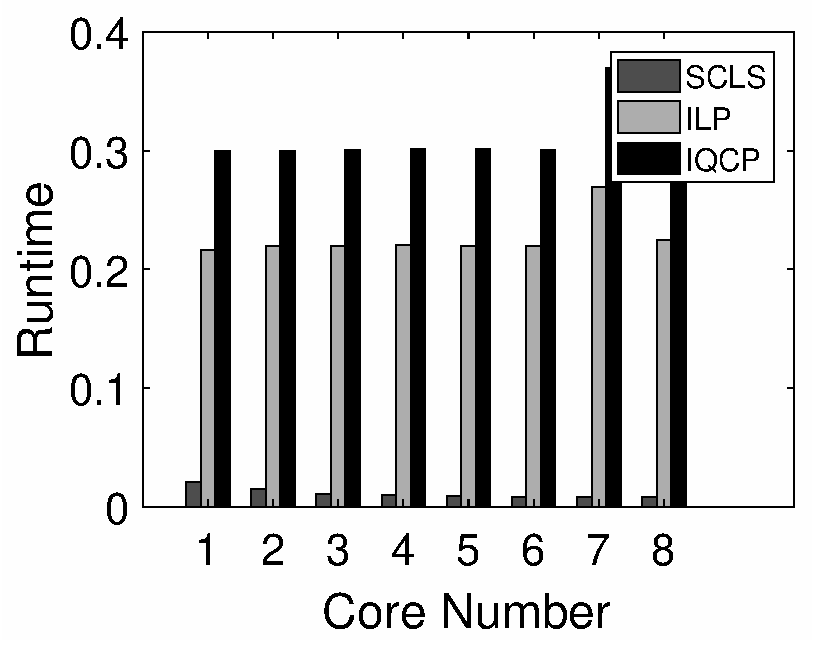
\includegraphics[width=2.25in]{figures/Runtime_noKSP_noCOSE}\\
  \caption{Runtime without CoSE}\label{fig:Runtime_noKSP_noCOSE}
\end{minipage}
\hfill
\begin{minipage}[t]{0.3\linewidth}
\centering
\includegraphics[width=2.25in]{figures/speedup}
\caption{Core speedup}
\label{fig:Speedup}
\end{minipage}
\end{figure*}


\begin{figure*}[tp]
\centering
\begin{minipage}[t]{0.3\linewidth}
\centering
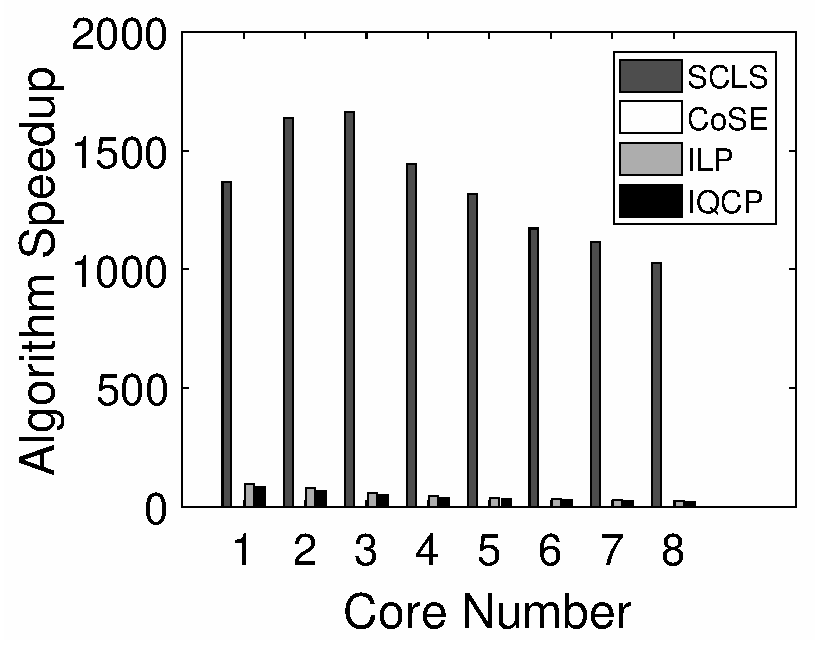
\includegraphics[width=2.25in]{figures/Multiple}
\caption{Algorithm speedup}
\label{fig:Multiple}
\end{minipage}
\hfill
\begin{minipage}[t]{0.3\linewidth}
\centering
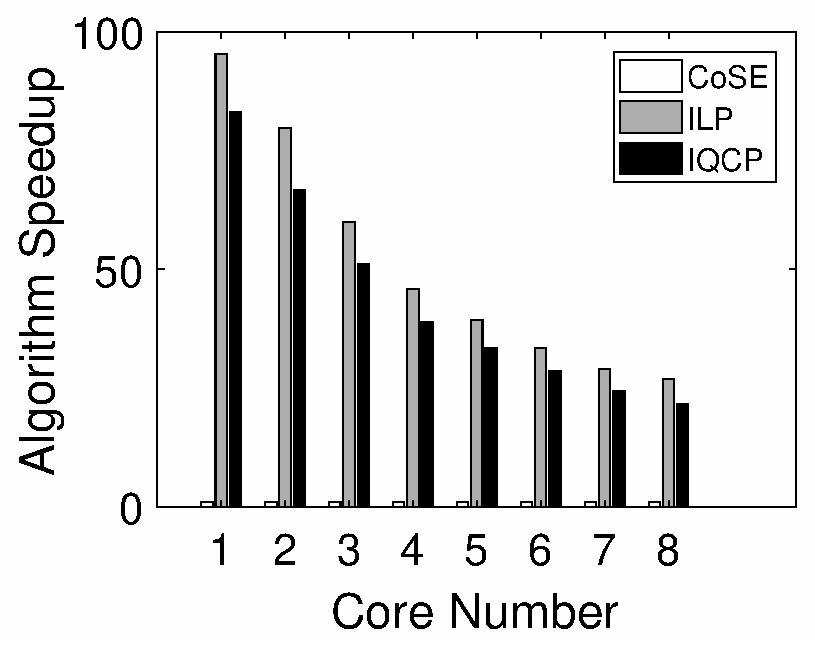
\includegraphics[width=2.25in]{figures/MultipleNoSCLS}
\caption{Algorithm speedup without SCLS}
\label{fig:MultipleNoSCLS}
\end{minipage}
\hfill
\begin{minipage}[t]{0.3\linewidth}
\centering
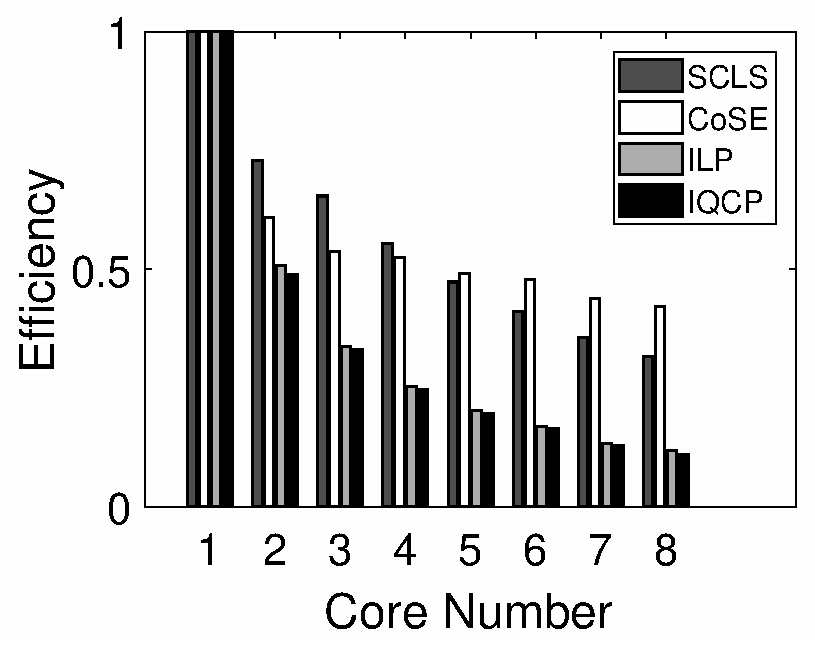
\includegraphics[width=2.25in]{figures/Efficiency}
 \caption{Efficiency}
 \label{fig:Efficiency}
\end{minipage}
\end{figure*}



\subsubsection{Path Hop}
Fig.\ref{fig:normalization hop} shows the path hop of AP, BP, and the sum of both AP and BP. As all algorithms target to minimize the least path weight of the SRLG-disjoint path pair instead of the number of path hops, they have the same AP weight (Fig.\ref{fig:normalization weitgh sum}) even though they have different AP path hops (Fig.\ref{fig:normalization hop}). Although the AP weights under all algorithms are smaller than the BP weights in Fig.\ref{fig:normalization weitgh sum}, in Fig.\ref{fig:normalization hop}, the AP hops may not always be fewer than the BP hops.

%\begin{figure}
%  \centering
%  % Requires \usepackage{graphicx}
%  \includegraphics[width=2.35in]{franz/hop}\\
%  \caption{Path hop}\label{fig:normalization hop}
%\end{figure}

尽管所有算法的AP权重都小于BP权重在图9中,在图10中,AP跳可能并不总是这样比英国石油公司的啤酒花还少。3)运行时:图11显示了不同运行时间下的运行时间算法通过改变CPU核的使用数量。如Cose下的运行时明显大于其他算法,以更清楚地显示其他算法的结果。算法,我们在图12中进一步绘制运行时结果因为ILP和IQCP不是并行算法,的不同数目下的这些算法的运行时。

\subsubsection{Runtime}
\label{subsubsec:Runtime}
Fig.\ref{fig:normalization runtime} shows the run time under different algorithms by varying the number of CPU cores utilized.
As the runtime under CoSE is significantly larger than that under other algorithms, to more clearly show the results of other algorithms, we further plot the runtime results in Fig.\ref{fig:Runtime_noKSP_noCOSE} by excluding CoSE.
As ILP, and IQCP are not parallel algorithms, the runtime of these algorithms under different number of cores is approximately equal. The runtime of our SCLS  and CoSE decreases with the increase of the number of processor cores because these two algorithms can partition the original problem into multiple sub-problems to execute in parallel and take advantage of the parallelism of the multi-core CPU to speed up the path searching process. Although CoSE is a parallel algorithm, the computation time is even larger than  ILP and IQCP. Some possible reasons include 1) the search process to find the conflicting SRLG set in CoSE  is not efficient; 2) As one SRLG usually includes multiple links, the partitioning of problem based on conflicting SRLG will introduce a large number of sub-problems to solve, which also results in a large computation cost.



%\begin{figure}
%  \centering
%  % Requires \usepackage{graphicx}
%  \includegraphics[width=2.35in]{franz/runtime}\\
%  \caption{Runtime}\label{fig:normalization runtime}
%\end{figure}
岩心大致相等。我们的SCLS和COSE随处理器数目的增加而减小。因为这两种算法可以分割原始的问题分成多个子问题并行执行利用多核CPU的并行性加快路径搜索过程。虽然Cose是并行算法,计算时间比ILP和IQCP。一些可能的原因包括:1)搜索在Cose中查找冲突的SRLG集的过程不是2)由于一个SRLG通常包含多个链接,基于冲突SRLG意志的问题划分介绍了大量的子问题需要解决,其中也有一些子问题需要解决。计算量大。与Cose不同的是,我们的SCLS寻找的是一组conf-将AP上的链接切换到陷阱问题中。图中的最小割集理论,实现了图的最短时间。图11。这表明我们的冲突链接集查找算法是有效的,而且我们的分而治之。基于SRLG的智能AP搜索过程及算法冲突链路集可以大大降低计算量。

Different from CoSE, our SCLS looks for the set of conflicting links on an AP caught into the trap problem based on the min-cut theory in graph, and achieves the lowest time in Fig.\ref{fig:normalization runtime}. This demonstrates that our conflicting link set finding algorithm is efficient, and moreover our divide-and-conquer algorithm and intelligent AP searching process based on SRLG Conflicting Link Set can largely reduce the computation cost.

%KSP is known as an effective algorithm to handle the trap problem. However, among all the algorithms implemented, the running time under KSP is the largest. A major problem of KSP is that after the current candidate AP fails the test (that is, it does not have a corresponding disjoint BP), the next candidate AP to be tested is selected solely based on the path length. In the 8 topologies we studied in the trace,  usually a large number of paths need to be tested in order to find a disjoint path pair (if it exists between a pair of nodes), thus KSP needs a large computation time.

\subsubsection{Algorithm speedup}
算法加速:在图14中,我们进一步比较了它们计算速度特别是,找出加速带在使用不同的算法查找所需的路径,我们使用Cose作为基线算法,并设置算法1。=Cose。类似于图11中的结果,SCLS的速度在图14中是Cose的700多倍。类似于图11,因为Cose的运行速度要小得多在图14中很难观察到,我们更进一步将图15中的算法加速比结果排除在最大的一次。

In Fig.\ref{fig:Multiple}, we further compare their computation speeds. Specially, to find out how much speedup is gained when using different algorithms to find the required paths,
%to calculate the algorithm speedup metric,
we use CoSE as the baseline algorithm and set $alg_1$ =CoSE. Similar to the results in the Fig.\ref{fig:normalization runtime}, the speed of SCLS is more than 700 times that of  CoSE in Fig.\ref{fig:Multiple}.  Similar to Fig.\ref{fig:normalization runtime}, as the running speed of CoSE is significantly smaller than others and can hardly be observed in Fig.\ref{fig:Multiple}, we further plot the algorithm speedup results in Fig.\ref{fig:MultipleNoSCLS} by excluding the largest one SCLS.



\subsubsection{Core speedup}

核心加速比:而不是使用算法加速若要比较所有算法的总体运行速度,请将使用公制“核心加速比”来评估数字的核心影响给定的运行速度。算法。图13绘制了所有算法下的核心加速图已执行。算法ILP和IQCP下的核心加速比是在任何核心数下大约等于1,因为它们不是并行算法。我们SCLS的核心加速当核数小于4时,随核心数的增加而增加,在此之后,SCLS的核心加速比保持稳定,即演示4核心对于SCLS来说是足够的。这个结果是符合Amdahl定律[41]的理论核心加速比仅限于由问题确定的上限。尺寸。然而,cose下的运行时继续增加。即使核心数等于8,这是双倍的。数字4。这个结果表明即使是8核cpu。不能满足COSE的并行性要求。这是因为Cose发现的冲突SRLG集包含一个大量的链接,这进一步导致了大量的链接子问题,因此问题的大小和计算量都很大。费用。


Rather than using the algorithm speedup to compare the overall running speeds of all algorithms, the metric "core speedup" is utilized to evaluate how the number of cores in the CPU impacts the running speed of a given algorithm.
Fig.\ref{fig:Speedup} plots the core speedup under all algorithms implemented.
%For the two parallel algorithms SCLS and CoSE, the core speedup   increases with the increase of the number of cores. %\del{Therefore, larger number of cores brings larger performance gain for these two parallel algorithms SCLS and CoSE.}
%However, the increasing speed becomes smaller when the number of cores becomes larger and it incurs a higher cost to coordinate the process.
Core speedup under algorithms ILP and IQCP is  approximately equal to 1 under any core number because they are not parallel algorithms. The core speedup of our SCLS increases with increase of core number when it is less than 4, beyond which the core speedup of SCLS remains stable, which demonstrates that 4 core is sufficient for SCLS. This result is consistent with Amdahl's law\cite{amdahl1967validity} that the theoretical core speedup is limited to a upper bound determined by the problem size. However, the runtime under CoSE continues to increases even though the core number is  equal to 8 which doubles the number 4. This result demonstrates that even 8-core CPU can not satisfy the parallelism requirement in CoSE. This is because the conflicting SRLG set found by CoSE includes  a large number of links,  which further results in a large number of sub-problems  and thus large problem size and  computation cost.


%1) the search
%process to find the conflicting SRLG set in CoSE is not
%efficient; 2) As one SRLG usually includes multiple links,
%the partitioning of problem based on conflicting SRLG will
%introduce a large number of sub-problems to solve, which also
%results in a large computation cost
%
%Among all algorithms, \revtao{the core speedup of our SCLS is the largest except CoSE, which demonstrates that our divide and conquer algorithm designed  based on the SRLG conflicting link set can bring the largest parallelism gain than non-parallel algorithm, and the cardinality of subproblem is smaller than CoSE}.

%\note{How many paths pairs to search in your simulations. If you only search for one pair, then the sub=-problems may be lower than the number of cores, so multi core cannot be used.}
\subsubsection{Efficiency}
%Efficiency is a measure of the overhead due to the parallelization. Programs with a high efficiency spend more time on useful work and less time on synchronization and communications.

效率:类似于图13,涉及更多的核心,效率值随着大量核心数的增加而降低。更多的成本来协调这一过程。在图16中,效率所有算法的值都随着核心号码。与图13中的结果一致,如Cose在核心之后,引入了比我们的scls更多的子问题。数达到4,在Cose下的效率大于。SCLS。然而,我们的SCLS取得了更大的成绩-如图14所示。所有的仿真结果表明,我们的SCLS可以实现。优于其他路由性能更高的方法而在更高的搜索速度,因为冲突找到的链接集可以促进有效的问题划分并行算法执行,计算量小。


Similar to Fig.\ref{fig:Speedup}, with more cores involved, the efficiency value decreases  as a large core number brings more cost to coordinate the process. In Fig.\ref{fig:Efficiency}, the efficiency values of all algorithms decrease with the increase of the core number. Consistent with the results in Fig.\ref{fig:Speedup}, as CoSE introduces more sub-problems than our SCLS, after the core number reaches 4, the efficiency under CoSE is larger than SCLS. However, our SCLS achieves significantly larger algorithm speedup as shown Fig.\ref{fig:Multiple}. %\note{You'd better use the same colore to represent the same algorithm in different figures. It makes reading and understanding difficult with your messy color setup. You may explain what is algorithm speedup and core speedup earlier when you first refer them, although you don't need to give formal definition.}

All the simulation results demonstrate that our SCLS can outperform other approaches with higher routing performance while at a much higher search speed, because the  conflicting link set found can facilitate efficient problem partition for parallel algorithm execution with low computation cost.


%\chapter{QoS约束下的链路分离路径问题研究}
\section{传统的QoS约束下的链路分离路径方法}
\section{算法性能评估}
\section{本章小节}
%% !Mode:: "TeX:UTF-8"

\chapter{总结和展望}
\section{本文工作总结}
本文在SDN/NFV架构下提出了两种故障情形下的可生存性算法。

首先,本文提出了一种拓扑图在存在陷阱问题情况下求解Min-Min SRLG不相交路由问题的高效算法。为了降低搜索的复杂性,我们创新性提出了一种分而治之的解决方案,将原Min-Min SRLG 不相交路由问题划分为多个子问题,该子问题基于从AP路径上遇到陷阱问题时导出的SRLG冲突链路集。我提出的算法利用现有的AP搜索结果和并行执行来实现更快的路径查找。并且在一个多核CPU平台上使用合成的拓扑进行了广泛的模拟。仿真结果表明,在搜索速度比较下,该算法的查找性能优于其它现有算法。

其次,本文在可生存性虚拟网络嵌入问题中,引入网络节点带有特定功能类型的限制条件,创新性提出一种星型分割动态分配嵌入的启发式算法,在虚拟和物理星型图之间的权重设置上,考虑网络资源的利用率和网络节点开启的代价。我提出的算法能快速的实现虚拟网络嵌入的可生存性需求,仿真结果表明,我提出的算法与其他现有算法效果比,虚拟嵌入可生存性请求的成功率更高,嵌入的物理资源消耗更低,物理资源的利用率更高。

\section{未来研究工作与展望}
未来对Min-Min SRLG不相交路由问题的研究中,可以考虑对路径权重的考虑涉及多属性多类型的考虑,而且不相交的条件涉及点边一同不相交的情形。对可生存性虚拟网络嵌入问题研究中,未来可以考虑对物理节点发生故障的情形,和考虑节点和链路更多的需求约束条件。
%结论应是作者在学位论文研究过程中所取得的创新性成果的概要总结,不能与摘要混为一谈。
%学位论文结论应包括论文的主要结果、创新点、展望三部分,在结论中应概括论文的核心观点,
%明确、客观地指出本研究内容的创新性成果(含新见解、新观点、方法创新、技术创新、理论创新),
%并指出今后进一步在本研究方向进行研究工作的展望与设想。
%对所取得的创新性成果应注意从定性和定量两方面给出科学、准确的评价,分(1)、(2)、(3)…条列出,宜用“提出了”、“建立了”等词叙述。



%\include{body/intros}
%\include{body/figures}
%\include{body/tables}
%\include{body/equations}
%\include{body/others}
%\section{conclusion}
\label{sec:conclusion}
%\del{In this paper, we have proved the Min-Min  SRLG-Disjoint routing problem is NP-complete.}
In this paper, we propose an efficient algorithm to solve the Min-Min  SRLG-Disjoint routing problem in the presence of the trap problem. To reduce the complexity of searching for the alternative pair, we propose a divide-and-conquer solution to partition the original Min-Min SRLG-Disjoint routing problem into multiple sub-problems based on a SRLG conflicting link set derived from the AP path encountering the trap problem. Our algorithm takes advantage of existing AP search results and parallel executions for significantly faster path finding.
We have conducted extensive simulations  using the topology trace  on a multi-core CPU platform. The simulation results demonstrate that our algorithm can outperform other approaches with higher routing performance while at a much higher search speed.
%\section*{Acknowledgment}
%%\end{spacing}
%The work is supported  by the  National Natural Science Foundation of China under Grant Nos.61572184, 61725206, 61472130, 61472131, and 61772191,  Hunan Provincial Natural Science Foundation of China under Grant No.2017JJ1010,  Science and Technology Key Projects of Hunan Province under Grant No.2015TP1004 and No.2016JC2012,  U.S. ONR N00014-17-1-2730, NSF ECCS 1408247, CNS 1526843, and ECCS 1731238.

%%%%%%%%%% 正文部分内容  %%%%%%%%%%

%%%%%%%%%%  参考文献  %%%%%%%%%%
\defaultfont
\bibliographystyle{HNUThesis}
\phantomsection
\addcontentsline{toc}{chapter}{参考文献}          % 参考文献加入到中文目录
%\nocite{*}                                        % 若将此命令屏蔽掉,则未引用的文献不会出现在文后的参考文献中。
\bibliography{reference}
% !Mode:: "TeX:UTF-8"
\addcontentsline{toc}{chapter}{致\quad 谢} %添加到目录中
\chapter*{致\quad 谢}
本论文的工作是在我的导师谢鲲教授的悉心指导下完成的,谢鲲教授严谨的写作态度和科学的工作方法给了我极大的帮助和影响。在此衷心感谢三年来谢老师对我的关心和指导。

%[XXXX...] 教授悉心指导我们完成了实验室的科研工作,在学习上和生活上都给予了我很大的关心和帮助,在此向[XXXX...] 老师表示衷心的谢意。

%[XXXX...] 教授对于我的科研工作和论文都提出了许多的宝贵意见,在此表示衷心的感谢。

在寝室工作及撰写论文期间,胡海洋 、何展等同学对我论文中的研究工作给予了热情帮助,在此向他们表达我的感激之情。

另外也感谢我家人和我的爱人,他们的理解和支持使我能够在学校专心完成我的学业。

其次,我想感谢我的学校、感谢湖南大学。惟楚有才、于斯为盛,有幸能够在千年学府里追溯着先贤的脚步,在这里度过人生中宝贵三年光阴。难忘的是那一场场湘江边盛大的烟火、那一次次呼朋引伴结伴而行的岳麓山之行,爱晚亭的枫、湘江的水还有那麓山南路的风,将永远流荡、吹拂在我的这颗心。


               % 致谢
\include{appendix/publications}                   % 发表论文和参加科研情况说明
\clearpage
\end{CJK*}                                        % 结束中文字体使用
\end{document}                                    % 结束全文
